\documentclass[aspectratio=169,12pt,t]{beamer}

% --- Theme: Metropolis (modern, clean) ---
\usetheme[progressbar=frametitle,numbering=fraction,block=fill]{metropolis}

% --- Fira Sans font (install texlive-fonts-extra if missing) ---
\IfFileExists{FiraSans.sty}{\usepackage[sfdefault]{FiraSans}}{}

% --- Light background with warm accent ---
\definecolor{mDarkTeal}{RGB}{35,55,59}
\definecolor{mLightBrown}{RGB}{235,228,216}
\definecolor{mAccent}{RGB}{140,70,20}

\setbeamercolor{normal text}{fg=mDarkTeal,bg=white}
\setbeamercolor{alerted text}{fg=mAccent}
\setbeamercolor{frametitle}{bg=mDarkTeal,fg=white}
\setbeamercolor{progress bar}{fg=mAccent,bg=mLightBrown}
\setbeamercolor{title separator}{fg=mAccent}
\setbeamercolor{progress bar in head/foot}{fg=mAccent,bg=mLightBrown}
\setbeamercolor{progress bar in section page}{fg=mAccent,bg=mLightBrown}

% --- Packages ---
\usepackage[utf8]{inputenc}
\usepackage{amsmath,amssymb,amsthm}
\usepackage{mathrsfs}
\usepackage{tikz}
\usetikzlibrary{arrows.meta,positioning,calc,decorations.pathreplacing,shapes,patterns,backgrounds,matrix}
\usepackage{pgfplots}
\pgfplotsset{compat=1.18}
\usepgfplotslibrary{fillbetween}

% --- TikZ diagram styles (shared across the series) ---
\tikzset{
  bgveil/.style={show background rectangle, inner frame sep=4pt,
    background rectangle/.style={fill=white, fill opacity=0.6, draw=none}},
  axisln/.style={-{Stealth[length=2.6mm]}, line width=0.8pt, gray!75},
  curveln/.style={line width=1.6pt, line cap=round, line join=round},
  projln/.style={dash pattern=on 2.6pt off 2pt, line width=0.7pt},
  guide/.style={-{Stealth[length=2.6mm,width=2.2mm]}, line width=1.1pt},
  box/.style={draw=#1, fill=#1!12, line width=1pt, rounded corners=2pt,
    minimum width=5.6cm, minimum height=1.35cm, align=center, font=\small},
  rbox/.style={box=#1, minimum width=0pt, text width=3.7cm},
}
% point marker with a white halo: \dotpt{color}{(coord)}
\newcommand{\dotpt}[2]{%
  \fill[white] #2 circle (3.6pt);
  \fill[#1] #2 circle (2.4pt);
}
% open point marker: \opendotpt{color}{(coord)}
\newcommand{\opendotpt}[2]{%
  \fill[white] #2 circle (3.6pt);
  \draw[#1, line width=1pt] #2 circle (2.4pt);
}

% --- Semi-transparent white highlight for text on top of background images ---
\usepackage[most]{tcolorbox}

% Inline highlight: \hl{short text}
\newtcbox{\hl}{%
  nobeforeafter, tcbox raise base,
  colback=white, opacityback=0.6,
  colframe=white, opacityframe=0,
  sharp corners, boxsep=2pt, left=3pt, right=3pt, top=2pt, bottom=2pt%
}

% Block highlight: \begin{hlbox} ... \end{hlbox}  (multi-line, paragraphs, itemize)
% Optional argument accepts any tcolorbox key, e.g. [width=0.6\linewidth]
\newtcolorbox{hlbox}[1][]{%
  enhanced, breakable,
  colback=white, opacityback=0.6,
  colframe=white, opacityframe=0,
  boxsep=3pt, left=6pt, right=6pt, top=4pt, bottom=4pt,
  sharp corners,
  {#1}%
}

% --- Custom colors for content types ---
\definecolor{defcolor}{RGB}{25,85,120}
\definecolor{thmcolor}{RGB}{140,35,35}
\definecolor{proofcolor}{RGB}{35,100,50}
\definecolor{excolor}{RGB}{140,75,10}
\definecolor{remcolor}{RGB}{90,90,90}

% --- Beamer blocks for mathematical content types (semi-transparent) ---
\tcbset{hlblockbase/.style={
  enhanced, breakable,
  coltitle=white, fonttitle=\bfseries,
  opacitybacktitle=0.8, opacityback=0.6,
  opacityframe=0,
  sharp corners,
  boxsep=1pt, left=5pt, right=5pt, top=2pt, bottom=2pt,
  toptitle=1pt, bottomtitle=1pt,
  before upper={\setlength{\abovedisplayskip}{4pt}\setlength{\belowdisplayskip}{4pt}}
}}

\newtcolorbox{defblock}[1]{hlblockbase, title={#1},
  colbacktitle=defcolor, colback=defcolor!15, colframe=defcolor}
\newtcolorbox{thmblock}[1]{hlblockbase, title={#1},
  colbacktitle=thmcolor, colback=thmcolor!15, colframe=thmcolor}
\newtcolorbox{proofblock}[1]{hlblockbase, title={#1},
  colbacktitle=proofcolor, colback=proofcolor!15, colframe=proofcolor}
\newtcolorbox{exblock}[1]{hlblockbase, title={#1},
  colbacktitle=excolor, colback=excolor!15, colframe=excolor}
\newtcolorbox{remblock}[1]{hlblockbase, title={#1},
  colbacktitle=remcolor, colback=remcolor!15, colframe=remcolor}


% --- Metadata ---
\title{Chapter 7: Sequences and Series of Functions}
\subtitle{Section: Equicontinuous Families of Functions}
\author{Based on Walter Rudin's \emph{Principles of Mathematical Analysis}}
\date{}

% --- Shared helpers for this deck ---
% Example 7.21: f_n(x) = x^2 / (x^2 + (1 - n x)^2)
\pgfmathdeclarefunction{spike}{2}{\pgfmathparse{(#1)^2/((#1)^2 + (1 - (#2)*(#1))^2)}}
% Compact set K used in the proof of Theorem 7.25
\newcommand{\Kblob}{%
  \draw[defcolor, line width=1.2pt, fill=defcolor!8]
    plot[smooth cycle, tension=0.75] coordinates
    {(-0.2,0.2) (1.3,-0.35) (2.9,-0.2) (3.9,0.6) (3.7,1.8) (2.4,2.25) (0.9,2.1) (-0.3,1.3)};
  \node[defcolor] at (4.25,2.1) {$K$};
}

\begin{document}

{
\usebackgroundtemplate{%
  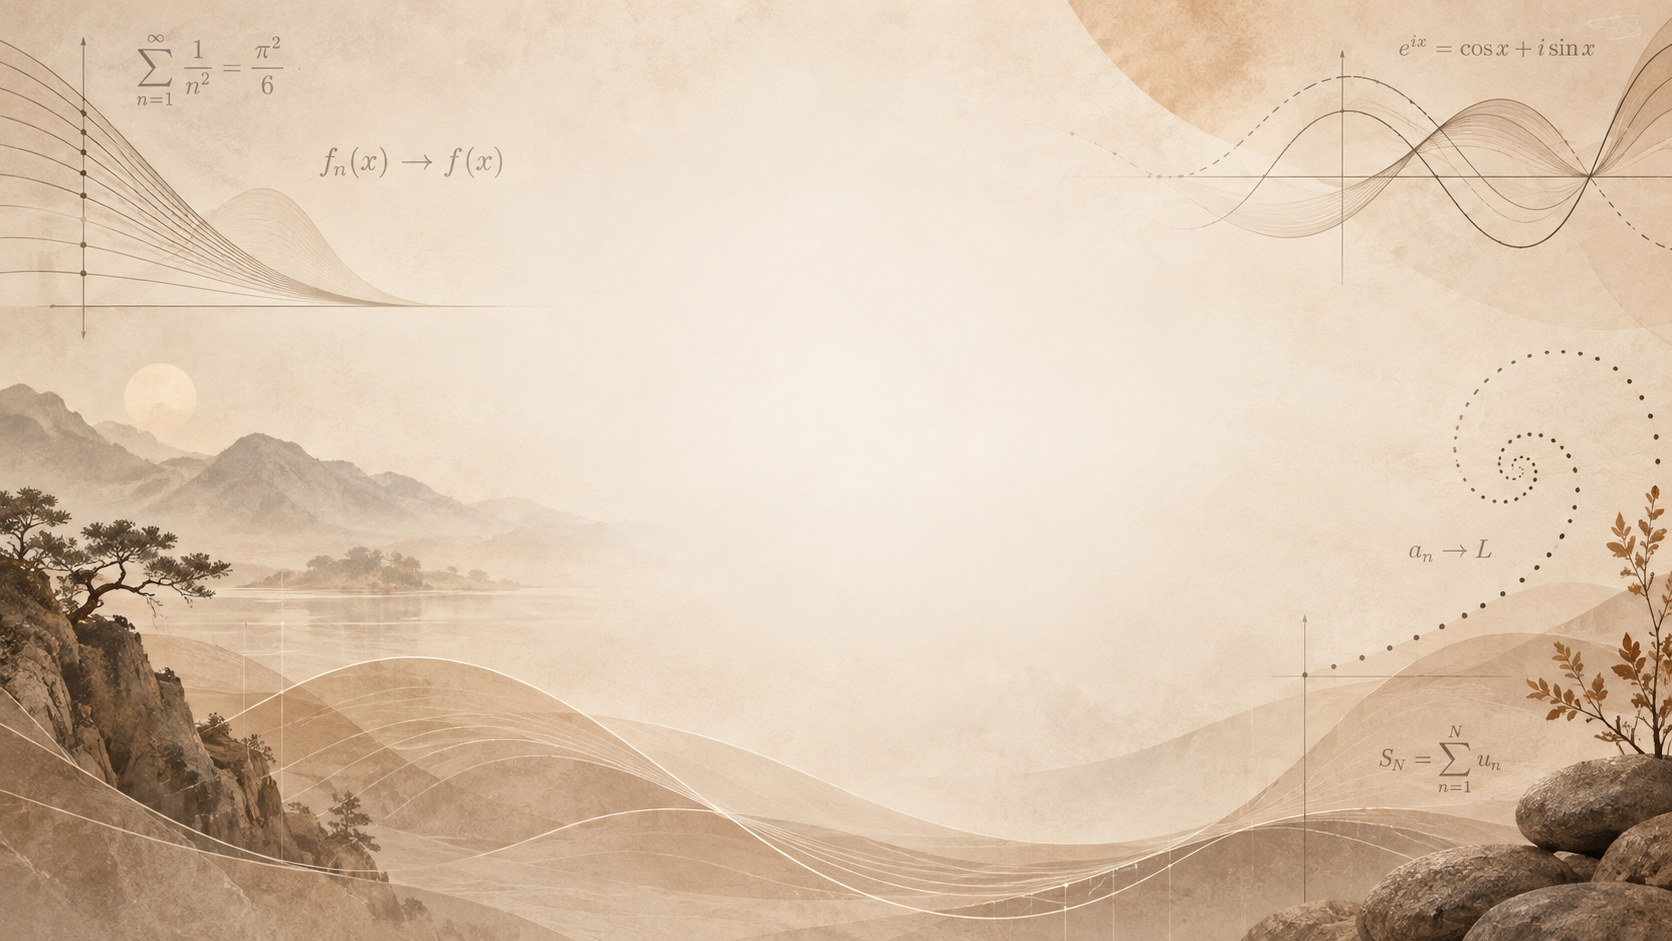
\includegraphics[width=\paperwidth,height=\paperheight,keepaspectratio=false]{chapter_07_bg_00.png}%
}
\begin{frame}[plain]
  \titlepage

  \note{
    Welcome back to Chapter 7, Sequences and Series of Functions. This
    is the sixth section, Equicontinuous Families of Functions. In
    Chapter 3 we learned that every bounded sequence of numbers has a
    convergent subsequence. In this section we ask whether something
    similar holds for sequences of functions. The answer requires a new
    idea, equicontinuity, and it culminates in a famous compactness
    theorem, usually called the Arzela Ascoli theorem. Let's begin.
  }
\end{frame}
}

{
\usebackgroundtemplate{%
  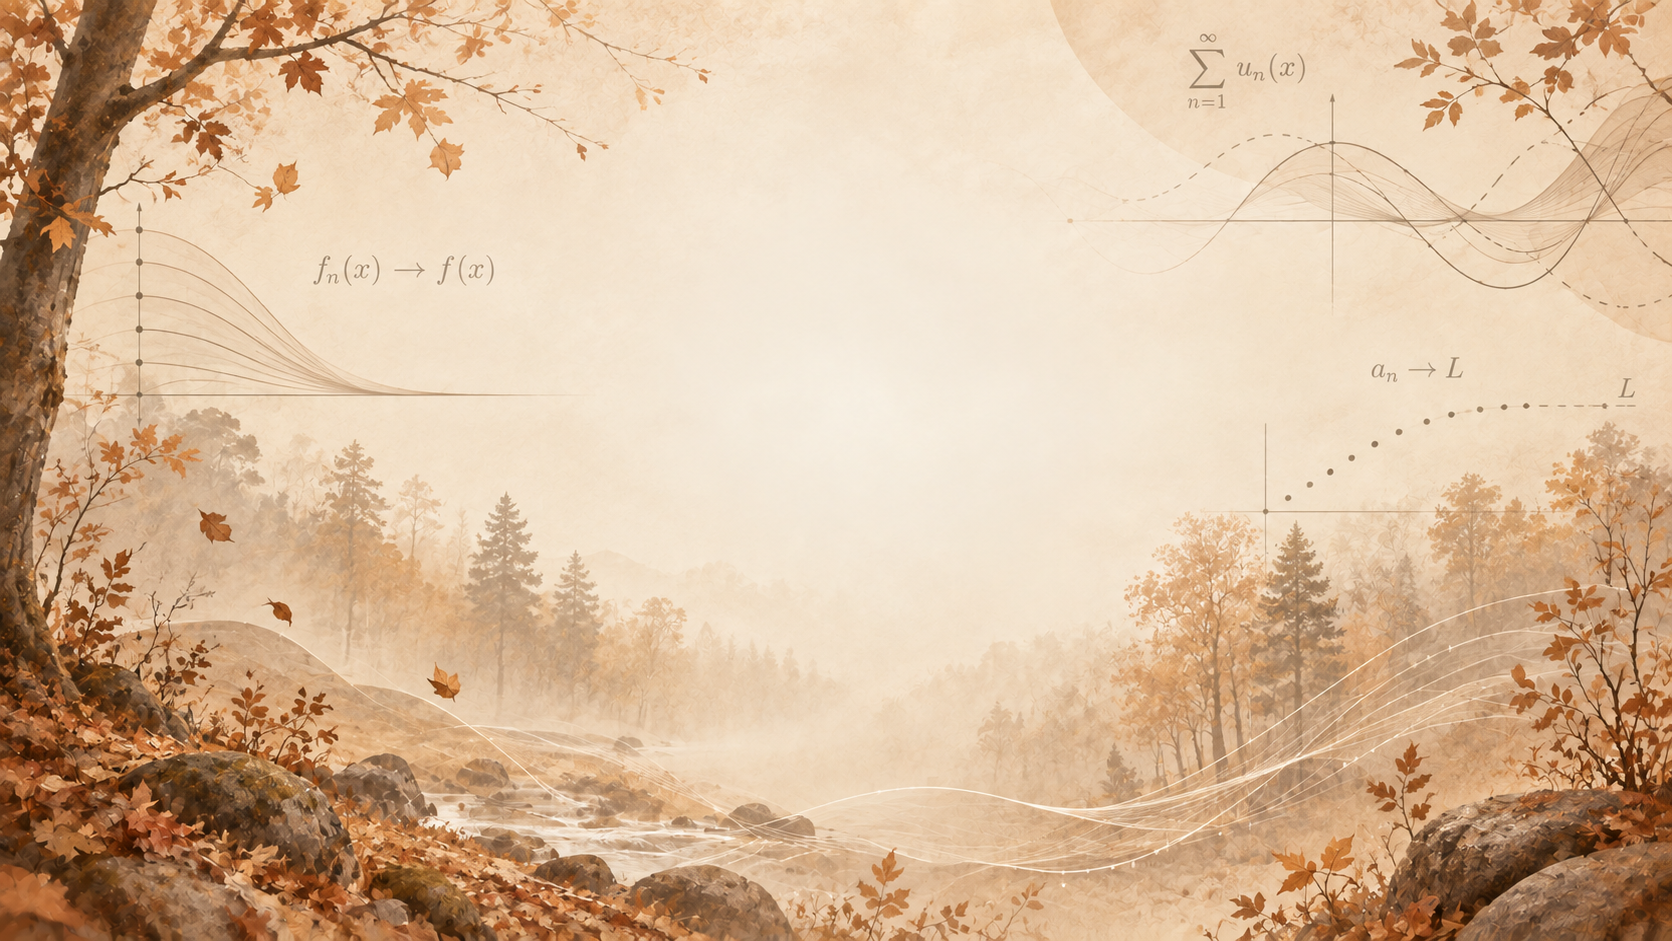
\includegraphics[width=\paperwidth,height=\paperheight,keepaspectratio=false]{chapter_07_bg_01.png}%
}
\begin{frame}[c]{Outline}
  \begin{center}
    \tableofcontents
  \end{center}

  \note{
    Here is the plan. After a short motivation, we define two kinds of
    boundedness for sequences of functions. Then come two cautionary
    examples, which show that boundedness alone is not enough. Next we
    introduce equicontinuity. We then prove a selection theorem using the
    diagonal process, show that uniform convergence implies
    equicontinuity, and finally prove the main theorem of the section,
    Theorem 7.25. We close with a summary.
  }
\end{frame}

\section{Motivation}

% --- Build 1/3 ---
\begin{frame}{Why This Section Matters}
  \begin{hlbox}
  \begin{itemize}
    \item \textbf{Theorem 3.6:} every \alert{bounded} sequence in $\mathbb{R}^k$
      has a \alert{convergent subsequence}
  \end{itemize}
  \end{hlbox}

  \note{
    Recall Theorem 3.6 from Chapter 3. It says that every bounded
    sequence of points in "k" dimensional Euclidean space contains a convergent subsequence. This
    is the Bolzano Weierstrass property, and we have used it again and
    again: to find limit points, to prove that continuous functions on
    compact sets attain their maximum, and much more. It is one of the
    most useful facts in analysis.
  }
\end{frame}

% --- Build 2/3 ---
\begin{frame}{Why This Section Matters}
  \begin{hlbox}
  \begin{itemize}
    \item \textbf{Theorem 3.6:} every \alert{bounded} sequence in $\mathbb{R}^k$
      has a \alert{convergent subsequence}
    \item \textbf{Question:} is the same true for a sequence of
      \emph{functions} $\{f_n\}$?
      \begin{itemize}
        \item What does ``bounded'' mean for $\{f_n\}$?
        \item Which kind of convergence do we want?
      \end{itemize}
  \end{itemize}
  \end{hlbox}

  \note{
    The natural question is whether something similar is true for
    sequences of functions. Before we can even ask it precisely, we have
    to decide two things, listed in the sub bullets. First, what should
    it mean for a sequence of functions to be bounded? Second, what kind
    of convergence do we want for the subsequence: pointwise convergence,
    or the much stronger uniform convergence?
  }
\end{frame}

% --- Build 3/3 ---
\begin{frame}{Why This Section Matters}
  \begin{hlbox}
  \begin{itemize}
    \item \textbf{Theorem 3.6:} every \alert{bounded} sequence in $\mathbb{R}^k$
      has a \alert{convergent subsequence}
    \item \textbf{Question:} is the same true for a sequence of
      \emph{functions} $\{f_n\}$?
      \begin{itemize}
        \item What does ``bounded'' mean for $\{f_n\}$?
        \item Which kind of convergence do we want?
      \end{itemize}
    \item \textbf{Answer (Theorem 7.25):} on a compact set, continuous $f_n$ that are
      pointwise bounded and \alert{equicontinuous} have a \alert{uniformly}
      convergent subsequence
  \end{itemize}
  \end{hlbox}

  \note{
    Here is a preview of the answer. Boundedness alone is not enough, as
    we will see in two examples. The missing ingredient is called
    equicontinuity. Theorem 7.25 shows that on a compact set, a sequence
    of continuous functions that is pointwise bounded and equicontinuous
    always has a uniformly convergent subsequence. That is the analogue
    of Theorem 3.6 for functions.
  }
\end{frame}

\begin{frame}{Roadmap of This Section}
  \vspace{0.6em}
  \begin{center}
  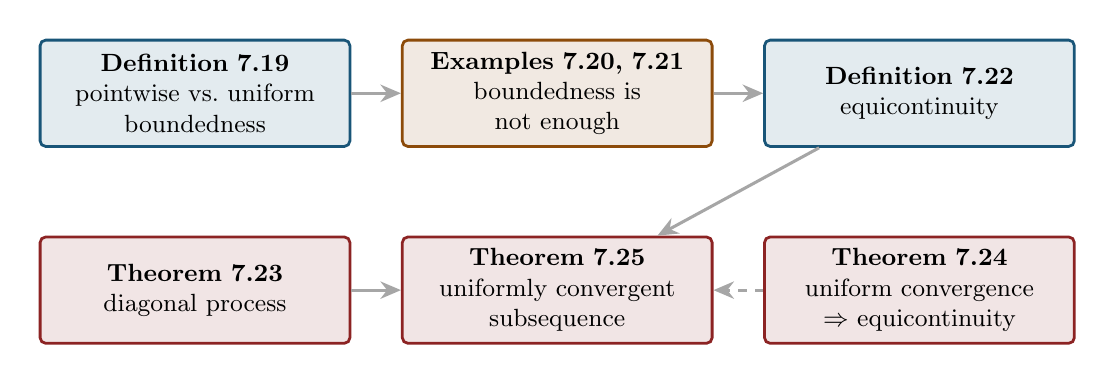
\begin{tikzpicture}[bgveil]
    \node[rbox=defcolor] (d1) at (-4.6,0) {\textbf{Definition 7.19}\\ pointwise vs.\ uniform\\ boundedness};
    \node[rbox=excolor] (e) at (0,0) {\textbf{Examples 7.20, 7.21}\\ boundedness is\\ not enough};
    \node[rbox=defcolor] (d2) at (4.6,0) {\textbf{Definition 7.22}\\ equicontinuity};
    \node[rbox=thmcolor] (t23) at (-4.6,-2.5) {\textbf{Theorem 7.23}\\ diagonal process};
    \node[rbox=thmcolor] (t24) at (4.6,-2.5) {\textbf{Theorem 7.24}\\ uniform convergence\\ $\Rightarrow$ equicontinuity};
    \node[rbox=thmcolor] (t25) at (0,-2.5) {\textbf{Theorem 7.25}\\ uniformly convergent\\ subsequence};
    \draw[guide, gray!70] (d1) -- (e);
    \draw[guide, gray!70] (e) -- (d2);
    \draw[guide, gray!70] (d2) -- (t25);
    \draw[guide, gray!70] (t23) -- (t25);
    \draw[guide, gray!70, dashed] (t24) -- (t25);
  \end{tikzpicture}
  \end{center}

  \note{
    The diagram shows how the section fits together. In the top row, in
    blue, Definition 7.19 introduces two kinds of boundedness. The brown
    box, Examples 7.20 and 7.21, shows that boundedness is not enough.
    That motivates the second blue box, Definition 7.22 of
    equicontinuity. In the bottom row, the red box on the left, Theorem
    7.23, is a selection result based on the diagonal process. Together
    with equicontinuity it feeds into the central red box, Theorem 7.25.
    On the right, Theorem 7.24 gives a partial converse, connected by the
    dashed arrow: uniform convergence forces equicontinuity.
  }
\end{frame}
}

{
\usebackgroundtemplate{%
  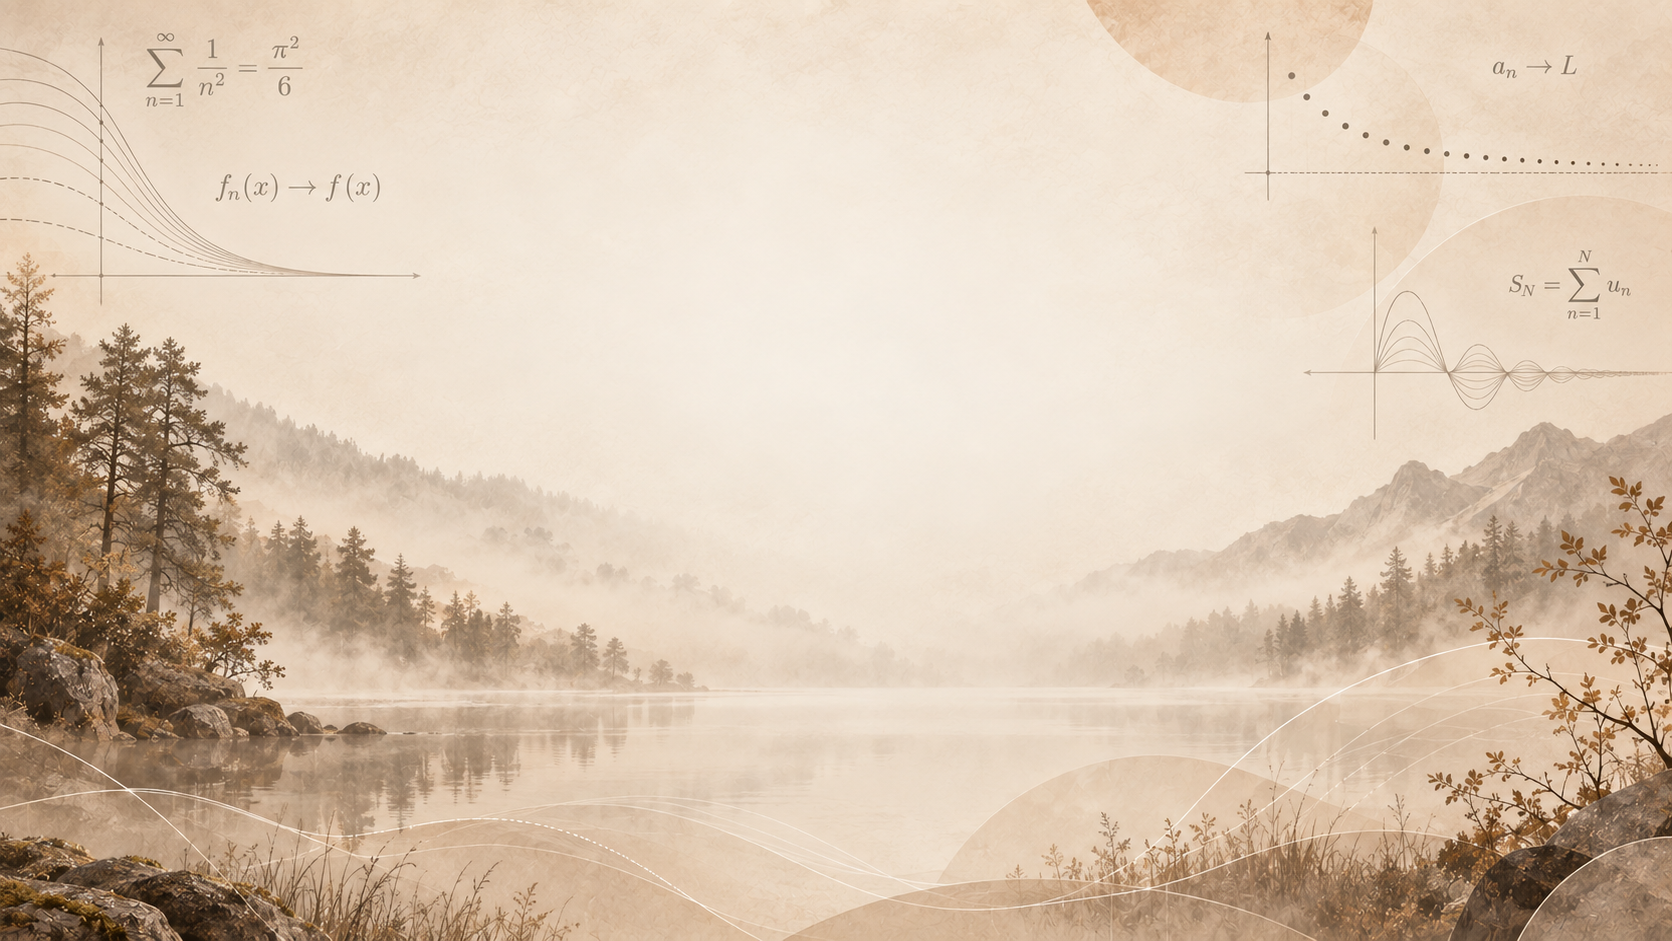
\includegraphics[width=\paperwidth,height=\paperheight,keepaspectratio=false]{chapter_07_bg_02.png}%
}
\section{Two Kinds of Boundedness}

% --- Build 1/2 ---
\begin{frame}{Definition 7.19: Pointwise and Uniform Boundedness}
  \begin{defblock}{Definition 7.19}
    Let $\{f_n\}$ be a sequence of functions defined on a set $E$.

    \medskip
    $\{f_n\}$ is \alert{pointwise bounded} on $E$ if $\{f_n(x)\}$ is bounded for
    every $x \in E$, i.e., there is a finite-valued function $\phi$ on $E$ with
    \[
      |f_n(x)| < \phi(x) \qquad (x \in E,\; n = 1, 2, 3, \dots).
    \]
  \end{defblock}

  \note{
    Here is the first kind of boundedness. A sequence "f" sub "n" is
    pointwise bounded on a set capital "E" if, at each fixed point "x",
    the sequence of numbers "f" sub "n" of "x" is bounded. The bound may
    depend on the point. We record it as a function phi, which must take
    finite values, and the inequality on the slide says that every "f"
    sub "n" stays below phi at every point. Notice that phi itself may be
    unbounded on capital "E".
  }
\end{frame}

% --- Build 2/2 ---
\begin{frame}{Definition 7.19: Pointwise and Uniform Boundedness}
  \begin{defblock}{Definition 7.19}
    Let $\{f_n\}$ be a sequence of functions defined on a set $E$.

    \medskip
    $\{f_n\}$ is \alert{pointwise bounded} on $E$ if $\{f_n(x)\}$ is bounded for
    every $x \in E$, i.e., there is a finite-valued function $\phi$ on $E$ with
    \[
      |f_n(x)| < \phi(x) \qquad (x \in E,\; n = 1, 2, 3, \dots).
    \]

    $\{f_n\}$ is \alert{uniformly bounded} on $E$ if there is a number $M$ with
    \[
      |f_n(x)| < M \qquad (x \in E,\; n = 1, 2, 3, \dots).
    \]
  \end{defblock}

  \note{
    The second kind is stronger. A sequence is uniformly bounded if a
    single number capital "M" works as a bound for all the functions at
    all the points at once. In other words, we may take phi to be a
    constant. Uniform boundedness implies pointwise boundedness, but not
    the other way around, as the next picture shows.
  }
\end{frame}

\begin{frame}{Pointwise vs.\ Uniform Boundedness}
  \begin{columns}[T]
    \begin{column}{0.5\textwidth}
      \centering
      \hl{\small\begin{tabular}{@{}c@{}}pointwise bounded:\\ $f_n(x) = \min(n, 1/x)$ on $(0,1]$\end{tabular}}\\[0.2em]
      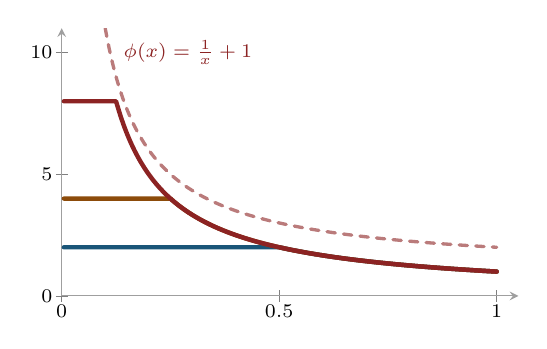
\begin{tikzpicture}
        \begin{axis}[
          axis background/.style={fill=white, fill opacity=0.6},
          scale only axis, width=5.8cm, height=3.4cm,
          xmin=0, xmax=1.05, ymin=0, ymax=11,
          axis x line=bottom, axis y line=left, axis line style={gray!75},
          xtick={0,0.5,1}, ytick={0,5,10},
          tick label style={font=\scriptsize, fill=white, fill opacity=0.6, text opacity=1, inner sep=1pt},
          every axis plot/.append style={curveln},
        ]
          \addplot[domain=0.1:1, samples=200, thmcolor!60, dashed, line width=1.2pt] {1/x + 1};
          \addplot[domain=0.005:1, samples=200, defcolor] {min(2, 1/x)};
          \addplot[domain=0.005:1, samples=200, excolor] {min(4, 1/x)};
          \addplot[domain=0.005:1, samples=300, thmcolor] {min(8, 1/x)};
          \node[thmcolor, font=\scriptsize, anchor=west] at (axis cs:0.12,10) {$\phi(x) = \tfrac1x + 1$};
        \end{axis}
      \end{tikzpicture}\\[0.2em]
      \hl{\small bounds grow near $0$: \alert{no single $M$}}
    \end{column}
    \begin{column}{0.5\textwidth}
      \centering
      \hl{\small\begin{tabular}{@{}c@{}}uniformly bounded:\\ $f_n(x) = \sin nx$ on $[0, 2\pi]$\end{tabular}}\\[0.2em]
      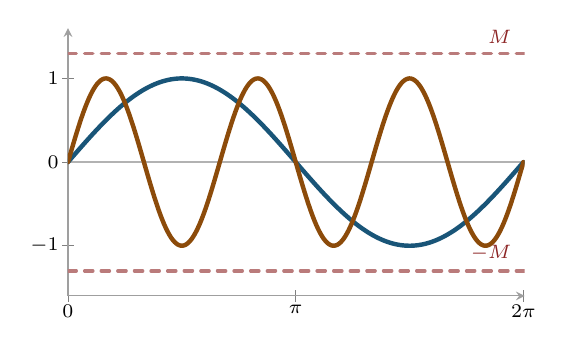
\begin{tikzpicture}
        \begin{axis}[
          axis background/.style={fill=white, fill opacity=0.6},
          scale only axis, width=5.8cm, height=3.4cm,
          xmin=0, xmax=6.3, ymin=-1.6, ymax=1.6,
          axis x line=bottom, axis y line=left, axis line style={gray!75},
          xtick={0,3.1416,6.2832}, xticklabels={$0$,$\pi$,$2\pi$},
          ytick={-1,0,1},
          tick label style={font=\scriptsize, fill=white, fill opacity=0.6, text opacity=1, inner sep=1pt},
          every axis plot/.append style={curveln},
        ]
          \draw[gray!60, line width=0.6pt] (axis cs:0,0) -- (axis cs:6.3,0);
          \addplot[domain=0:6.3, samples=2, thmcolor!60, dashed, line width=1.2pt] {1.3};
          \addplot[domain=0:6.3, samples=2, thmcolor!60, dashed, line width=1.2pt] {-1.3};
          \addplot[domain=0:6.2832, samples=200, defcolor] {sin(deg(x))};
          \addplot[domain=0:6.2832, samples=300, excolor] {sin(deg(3*x))};
          \node[thmcolor, font=\scriptsize, anchor=south east] at (axis cs:6.25,1.3) {$M$};
          \node[thmcolor, font=\scriptsize, anchor=south east] at (axis cs:6.25,-1.3) {$-M$};
        \end{axis}
      \end{tikzpicture}\\[0.2em]
      \hl{\small one constant $M$ works \alert{everywhere}}
    \end{column}
  \end{columns}

  \note{
    Two pictures contrast the definitions. On the left, on the interval
    from 0 to 1 with the point zero left out, we see the functions "f" sub
    "n" equal to the minimum of "n" and one over "x", for "n" equal to 2
    in blue, 4 in brown, and 8 in red. Each function is bounded, and at
    each point "x" all of them stay below the dashed red curve phi, one
    over "x" plus one. The plus one is there because the definition asks
    for a strict inequality. So the sequence is pointwise bounded. But
    near zero the bounds blow up, so no single constant works. On the
    right are the functions sine of "x" in blue and sine of 3 "x" in
    brown. They all stay between the dashed lines at capital "M" and minus
    capital "M", with capital "M" any number above 1, so this sequence is
    uniformly bounded.
  }
\end{frame}

% --- Build 1/2 ---
\begin{frame}{What Can Boundedness Buy Us?}
  \begin{remblock}{Countably many points: always possible}
    If $\{f_n\}$ is pointwise bounded on $E$ and $E_1 \subset E$ is
    \alert{countable}, there is a subsequence $\{f_{n_k}\}$ with
    \[
      \{f_{n_k}(x)\} \text{ convergent for every } x \in E_1.
    \]
    (Diagonal process, proof of Theorem 7.23.)
  \end{remblock}

  \note{
    What can boundedness alone give us? Quite a lot on a countable set.
    If the sequence is pointwise bounded on capital "E", and capital "E"
    sub 1 is a countable subset, we can always pick a subsequence that
    converges at every point of capital "E" sub 1. At a single point
    this is just Theorem 3.6. The trick for handling countably many
    points at once is called the diagonal process, and we will see it in
    detail in the proof of Theorem 7.23.
  }
\end{frame}

% --- Build 2/2 ---
\begin{frame}{What Can Boundedness Buy Us?}
  \begin{remblock}{Countably many points: always possible}
    If $\{f_n\}$ is pointwise bounded on $E$ and $E_1 \subset E$ is
    \alert{countable}, there is a subsequence $\{f_{n_k}\}$ with
    \[
      \{f_{n_k}(x)\} \text{ convergent for every } x \in E_1.
    \]
    (Diagonal process, proof of Theorem 7.23.)
  \end{remblock}

  \begin{remblock}{All points: may fail}
    Even if $\{f_n\}$ is a \emph{uniformly bounded} sequence of
    \emph{continuous} functions on a \emph{compact} set $E$, there need
    \alert{not} be a subsequence converging pointwise on $E$.
  \end{remblock}

  \note{
    On an uncountable set, however, the situation changes completely.
    The second box says that even with every hypothesis we could wish
    for, a uniformly bounded sequence of continuous functions on a
    compact set, there may be no subsequence that converges at every
    point. The next example proves this. Rudin remarks that the proof
    would be hard with our current tools, but becomes simple with a
    theorem from Chapter 11.
  }
\end{frame}
}

{
\usebackgroundtemplate{%
  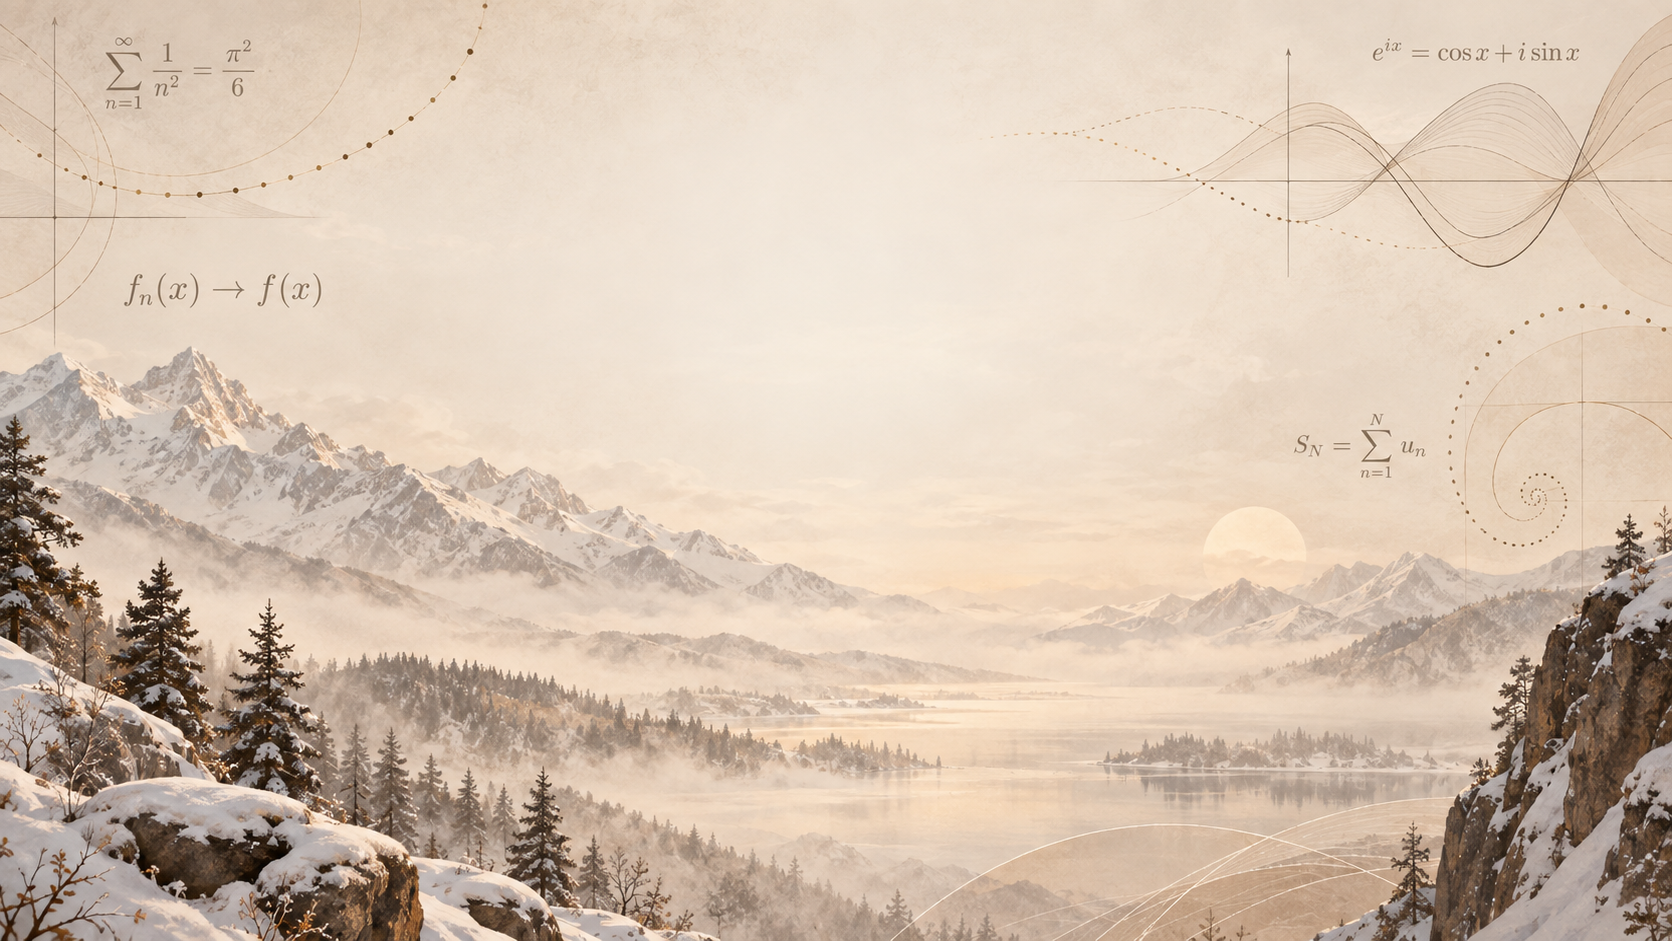
\includegraphics[width=\paperwidth,height=\paperheight,keepaspectratio=false]{chapter_07_bg_03.png}%
}
\section{Two Cautionary Examples}

\begin{frame}{Example 7.20: $\sin nx$ Has No Pointwise Convergent Subsequence}
  \begin{exblock}{Example 7.20}
    \[
      f_n(x) = \sin nx \qquad (0 \le x \le 2\pi,\; n = 1, 2, 3, \dots)
    \]
    is uniformly bounded ($|f_n| \le 1$) and continuous on the compact set
    $[0, 2\pi]$, but \alert{no subsequence} converges at every point.
  \end{exblock}

  \vspace{-0.3em}
  \begin{center}
  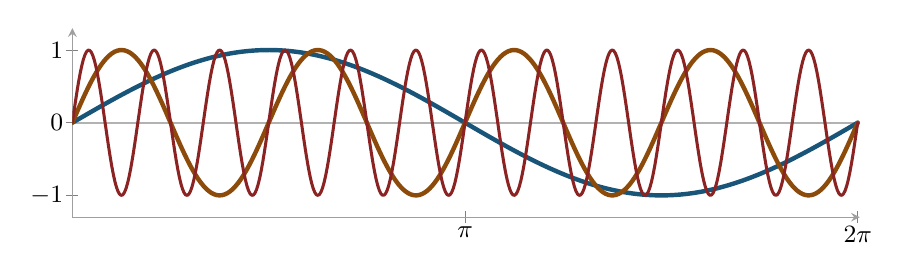
\begin{tikzpicture}
    \begin{axis}[
      axis background/.style={fill=white, fill opacity=0.6},
      scale only axis, width=10cm, height=2.4cm,
      xmin=0, xmax=6.3, ymin=-1.3, ymax=1.3,
      axis x line=bottom, axis y line=left, axis line style={gray!75},
      xtick={3.1416,6.2832}, xticklabels={$\pi$,$2\pi$},
      ytick={-1,0,1},
      tick label style={font=\small, fill=white, fill opacity=0.6, text opacity=1, inner sep=1pt},
      every axis plot/.append style={curveln},
    ]
      \draw[gray!60, line width=0.6pt] (axis cs:0,0) -- (axis cs:6.3,0);
      \addplot[domain=0:6.2832, samples=200, defcolor] {sin(deg(x))};
      \addplot[domain=0:6.2832, samples=300, excolor] {sin(deg(4*x))};
      \addplot[domain=0:6.2832, samples=500, thmcolor, line width=1.1pt] {sin(deg(12*x))};
    \end{axis}
  \end{tikzpicture}\\[0.1em]
  \hl{\small \textcolor{defcolor}{$n=1$} \quad \textcolor{excolor}{$n=4$} \quad \textcolor{thmcolor}{$n=12$}}
  \end{center}

  \note{
    Here is the example. The functions are sine of "n" "x" on the
    interval from 0 to 2 pi. They are continuous, the interval is
    compact, and they are all bounded by 1, so the sequence is uniformly
    bounded. The plot shows "n" equal to 1 in blue, 4 in brown, and 12 in
    red. As "n" grows, the waves oscillate faster and faster, and it is
    plausible that no subsequence can settle down at every point. Let's
    prove it.
  }
\end{frame}

% --- Build 1/3 ---
\begin{frame}{Example 7.20: Proof}
  \hl{\textbf{Technique:} Proof by contradiction.}

  \begin{proofblock}{Suppose $\{\sin n_k x\}$ converges for every $x \in [0, 2\pi]$}
    Consecutive terms of a convergent sequence get close, so
    \[
      \lim_{k \to \infty} (\sin n_k x - \sin n_{k+1} x)^2 = 0
      \qquad (0 \le x \le 2\pi). \tag{40}
    \]
  \end{proofblock}

  \note{
    We argue by contradiction. Suppose some subsequence, with indices
    "n" sub "k", converges at every point of the interval. Then, at each
    point, the difference between two consecutive terms tends to zero,
    and so does its square. That is equation 40. Squaring may look
    pointless, but it prepares us to integrate: a square is nonnegative
    and easy to integrate exactly.
  }
\end{frame}

% --- Build 2/3 ---
\begin{frame}{Example 7.20: Proof}
  \hl{\textbf{Technique:} Proof by contradiction.}

  \begin{proofblock}{Suppose $\{\sin n_k x\}$ converges for every $x \in [0, 2\pi]$}
    Consecutive terms of a convergent sequence get close, so
    \[
      \lim_{k \to \infty} (\sin n_k x - \sin n_{k+1} x)^2 = 0
      \qquad (0 \le x \le 2\pi). \tag{40}
    \]
    The integrands are bounded by $4$, so by \alert{Lebesgue's bounded
    convergence theorem} (Theorem 11.32), (40) implies
    \[
      \lim_{k \to \infty} \int_0^{2\pi} (\sin n_k x - \sin n_{k+1} x)^2\,dx = 0. \tag{41}
    \]
  \end{proofblock}

  \note{
    Now comes the step that needs Chapter 11. The functions in equation
    40 are all bounded by 4 and converge to zero at every point. Lebesgue's
    theorem on boundedly convergent sequences, Theorem 11.32, says that in
    this situation we may pass the limit inside the integral. Note that
    we only have pointwise convergence here, so the uniform convergence
    results of this chapter would not apply. The conclusion is equation
    41: the integrals tend to zero.
  }
\end{frame}

% --- Build 3/3 ---
\begin{frame}{Example 7.20: Proof}
  \hl{\textbf{So far:} (41) says the integrals of $(\sin n_k x - \sin n_{k+1} x)^2$ tend to $0$.}

  \begin{proofblock}{But a direct computation gives (for $m \ne n$ positive integers)}
    \[
      \int_0^{2\pi} (\sin mx - \sin nx)^2\,dx
      = \underbrace{\int_0^{2\pi}\!\sin^2 mx}_{\pi}
      + \underbrace{\int_0^{2\pi}\!\sin^2 nx}_{\pi}
      - 2\underbrace{\int_0^{2\pi}\!\sin mx \sin nx}_{0}
      = 2\pi.
    \]
    With $m = n_k$, $n = n_{k+1}$, every integral in (41) equals
    $2\pi$ --- \alert{contradiction!}
  \end{proofblock}

  \vspace{0.3em}
  \begin{center}
    \hl{$\boxed{\text{No subsequence of } \{\sin nx\} \text{ converges pointwise on } [0, 2\pi].}$}
  \end{center}

  \note{
    The line at the top recalls equation 41: these integrals must tend to
    zero. But we can compute them exactly. Expanding the square gives
    three pieces. Over the interval from 0 to 2 pi, the integral of sine
    squared of "m" "x" is pi, and so is the integral of sine squared of
    "n" "x". The cross term vanishes, because sines with different
    frequencies are orthogonal on this interval. So every integral equals
    2 pi, which certainly does not tend to zero. This contradicts equation
    41, and the boxed conclusion follows: no subsequence of sine of "n"
    "x" converges at every point.
  }
\end{frame}

\begin{frame}{A Second Question}
  \begin{hlbox}
  \begin{itemize}
    \item \textbf{Question:} does every \emph{convergent} sequence contain a
      \alert{uniformly convergent} subsequence?
    \item \textbf{No} --- not even if it is uniformly bounded on a compact
      set (Example 7.21).
  \end{itemize}
  \end{hlbox}

  \vspace{0.3em}
  \begin{remblock}{Remark}
    \begin{itemize}
      \item Example 7.6: bounded functions may \emph{converge} without being
        uniformly bounded.
      \item But $f_n \to f$ \emph{uniformly}, each $f_n$ bounded
        $\;\Longrightarrow\;$ $\{f_n\}$ \alert{uniformly bounded}.
    \end{itemize}
  \end{remblock}

  \note{
    Here is a second, more modest question. Suppose a sequence already
    converges pointwise. Can we always extract a uniformly convergent
    subsequence? The answer is again no, even for a uniformly bounded
    sequence on a compact set, as the next example shows. The gray box
    adds a side remark. In Example 7.6, the functions are "n" squared
    times "x", times the quantity one minus "x" squared, raised to the
    power "n". They converge to zero pointwise but are not uniformly
    bounded. On the other hand, a uniform limit of bounded functions is
    always uniformly bounded: beyond some index all the functions are
    within 1 of a single bounded function, and the first finitely many are
    bounded anyway.
  }
\end{frame}

% --- Build 1/3 ---
\begin{frame}{Example 7.21: No Uniformly Convergent Subsequence}
  \begin{exblock}{Example 7.21}
    \[
      f_n(x) = \frac{x^2}{x^2 + (1 - nx)^2} \qquad (0 \le x \le 1,\; n = 1, 2, 3, \dots).
    \]
  \end{exblock}

  \begin{center}
  \begin{tikzpicture}
    \begin{axis}[
      axis background/.style={fill=white, fill opacity=0.6},
      scale only axis, width=10cm, height=2.5cm,
      xmin=0, xmax=1.02, ymin=0, ymax=1.18,
      axis x line=bottom, axis y line=left, axis line style={gray!75},
      xtick={0,0.1,0.25,0.5,1}, xticklabels={$0$,$\tfrac1{10}$,$\tfrac14$,$\tfrac12$,$1$},
      ytick={0.5,1},
      tick label style={font=\scriptsize, fill=white, fill opacity=0.6, text opacity=1, inner sep=1pt},
      every axis plot/.append style={curveln},
    ]
      \addplot[domain=0:1, samples=300, defcolor] {spike(x,2)};
      \addplot[domain=0:1, samples=400, excolor] {spike(x,4)};
      \addplot[domain=0:1, samples=900, thmcolor] {spike(x,10)};
    \end{axis}
  \end{tikzpicture}\\[0.1em]
  \hl{\small \textcolor{defcolor}{$n=2$} \quad \textcolor{excolor}{$n=4$} \quad \textcolor{thmcolor}{$n=10$}}
  \end{center}

  \note{
    Here is the example. Each function "f" sub "n" is a quotient whose
    denominator is "x" squared plus one minus "n" "x", squared. The plot
    shows "n" equal to 2 in blue, 4 in brown, and 10 in red. Each graph
    is a spike that reaches height 1 at the point one over "n", and the
    spikes become narrower and move toward zero as "n" grows. Away from
    the spike each function is small.
  }
\end{frame}

% --- Build 2/3 ---
\begin{frame}{Example 7.21: No Uniformly Convergent Subsequence}
  \begin{exblock}{Example 7.21}
    \[
      f_n(x) = \frac{x^2}{x^2 + (1 - nx)^2} \qquad (0 \le x \le 1,\; n = 1, 2, 3, \dots).
    \]
    \begin{itemize}
      \item $|f_n(x)| \le 1$ $\;\Rightarrow\;$ \alert{uniformly bounded} on $[0,1]$
      \item $\displaystyle \lim_{n \to \infty} f_n(x) = 0$ for every $x \in [0,1]$
    \end{itemize}
  \end{exblock}

  \note{
    Two facts are easy. The numerator never exceeds the denominator, so
    every "f" sub "n" lies between 0 and 1, and the sequence is uniformly
    bounded. Also the sequence converges to zero at every point. At "x"
    equal to zero every term is zero. For a fixed positive "x", the second
    part of the denominator, one minus "n" "x", squared, grows like "n"
    squared, while the numerator stays fixed, so the quotient goes to
    zero.
  }
\end{frame}

% --- Build 3/3 ---
\begin{frame}{Example 7.21: No Uniformly Convergent Subsequence}
  \begin{exblock}{Example 7.21}
    \[
      f_n(x) = \frac{x^2}{x^2 + (1 - nx)^2} \qquad (0 \le x \le 1,\; n = 1, 2, 3, \dots).
    \]
    \begin{itemize}
      \item $|f_n(x)| \le 1$ $\;\Rightarrow\;$ \alert{uniformly bounded} on $[0,1]$
      \item $\displaystyle \lim_{n \to \infty} f_n(x) = 0$ for every $x \in [0,1]$
      \item But $f_n\!\left(\tfrac1n\right) = 1$ for all $n$, so
        $\sup_{[0,1]} |f_n - 0| = 1 \not\to 0$
    \end{itemize}
  \end{exblock}

  \vspace{0.2em}
  \begin{center}
    \hl{$\boxed{\text{No subsequence of } \{f_n\} \text{ converges uniformly on } [0,1].}$}
  \end{center}

  \note{
    But at the point one over "n" the second term in the denominator
    vanishes, and "f" sub "n" equals exactly 1. So the supremum of "f" sub
    "n" over the interval is always 1. If a subsequence converged
    uniformly, its limit would have to be the pointwise limit, which is
    zero, and the suprema would have to tend to zero. They do not. So no
    subsequence converges uniformly. The concept that rules out such
    moving spikes is equicontinuity, which we define next.
  }
\end{frame}
}

{
\usebackgroundtemplate{%
  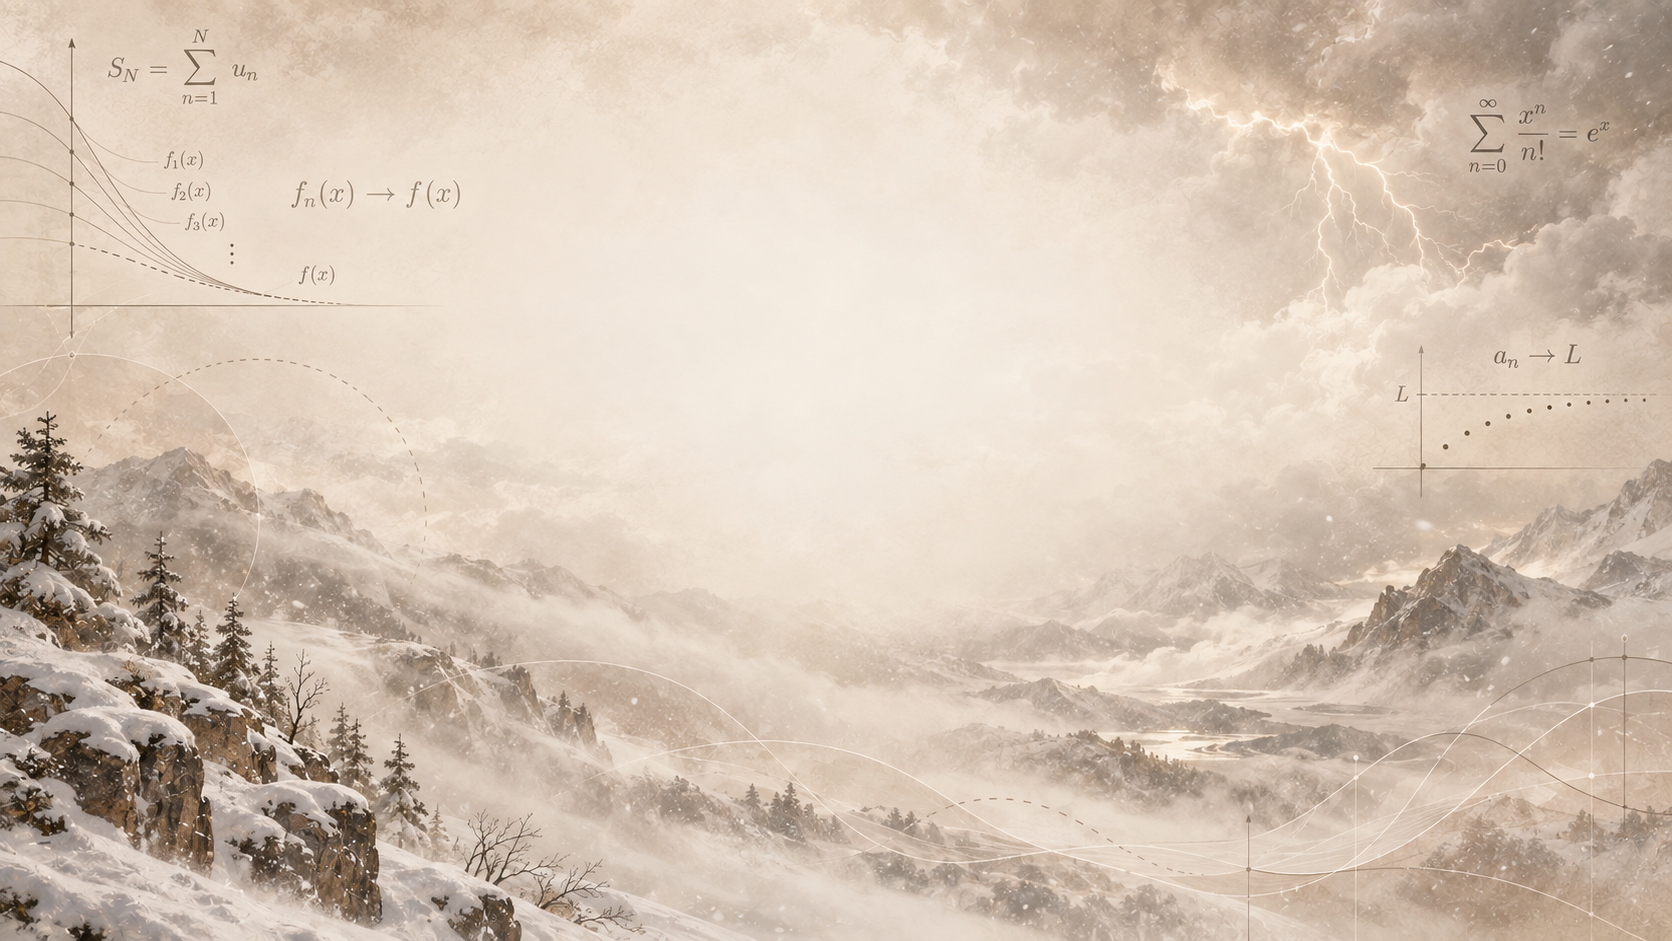
\includegraphics[width=\paperwidth,height=\paperheight,keepaspectratio=false]{chapter_07_bg_04.png}%
}
\section{Equicontinuity}

% --- Build 1/2 ---
\begin{frame}{Definition 7.22: Equicontinuity}
  \begin{defblock}{Definition 7.22}
    A family $\mathscr{F}$ of complex functions $f$ defined on a set $E$ in a
    metric space $X$ is \alert{equicontinuous} on $E$ if for every
    $\varepsilon > 0$ there exists a $\delta > 0$ such that
    \[
      |f(x) - f(y)| < \varepsilon
    \]
    whenever $d(x, y) < \delta$, $x \in E$, $y \in E$, and
    $f \in \mathscr{F}$. ($d$ is the metric of $X$.)
  \end{defblock}

  \note{
    Here is the key definition. A family of functions, written with a
    script capital "F", is equicontinuous on capital "E" if, for every
    positive epsilon, there is a positive delta such that any two points
    closer than delta have function values closer than epsilon. Distance
    is measured by "d", the metric of the space capital "X". The crucial
    point is the last condition: this must hold for every function "f" in
    the family, with one and the same delta.
  }
\end{frame}

% --- Build 2/2 ---
\begin{frame}{Definition 7.22: Equicontinuity}
  \begin{defblock}{Definition 7.22}
    A family $\mathscr{F}$ of complex functions $f$ defined on a set $E$ in a
    metric space $X$ is \alert{equicontinuous} on $E$ if for every
    $\varepsilon > 0$ there exists a $\delta > 0$ such that
    \[
      |f(x) - f(y)| < \varepsilon
    \]
    whenever $d(x, y) < \delta$, $x \in E$, $y \in E$, and
    $f \in \mathscr{F}$. ($d$ is the metric of $X$.)
  \end{defblock}

  \vspace{0.2em}
  \begin{hlbox}
  {\small
  \begin{tabular}{@{}ll@{}}
    \textbf{Uniform continuity of each $f$:} &
      $\forall f\;\; \forall \varepsilon\;\; \exists \delta = \delta(\varepsilon, \alert{f})\;\; \forall x, y$\\[0.3em]
    \textbf{Equicontinuity of $\mathscr{F}$:} &
      $\forall \varepsilon\;\; \exists \delta = \delta(\varepsilon)\;\; \alert{\forall f}\;\; \forall x, y$
  \end{tabular}}
  \end{hlbox}

  \note{
    The two lines below the box compare the order of the quantifiers. If
    each function is uniformly continuous, then for each function "f" and
    each epsilon we get a delta, but that delta may depend on "f", as the
    orange highlight shows. Equicontinuity moves the quantifier over the
    functions after the choice of delta: one delta must serve the whole
    family. So equicontinuity is uniform continuity that is also uniform
    across the family.
  }
\end{frame}

\begin{frame}{One $\delta$ for the Whole Family}
  \begin{columns}[T]
    \begin{column}{0.5\textwidth}
      \centering
      \hl{\small $\{\sin(x + c)\}$: \alert{equicontinuous}}\\[0.2em]
      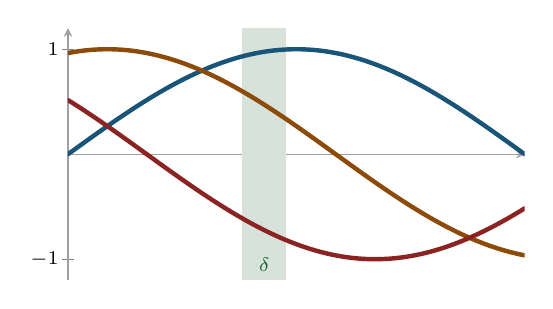
\begin{tikzpicture}
        \begin{axis}[
          axis background/.style={fill=white, fill opacity=0.6},
          scale only axis, width=5.8cm, height=3.2cm,
          xmin=0, xmax=3.1416, ymin=-1.2, ymax=1.2,
          axis x line=middle, axis y line=left, axis line style={gray!75},
          xtick=\empty, ytick={-1,1},
          tick label style={font=\scriptsize, fill=white, fill opacity=0.6, text opacity=1, inner sep=1pt},
          every axis plot/.append style={curveln},
        ]
          \fill[proofcolor!18] (axis cs:1.2,-1.2) rectangle (axis cs:1.5,1.2);
          \addplot[domain=0:3.1416, samples=150, defcolor] {sin(deg(x))};
          \addplot[domain=0:3.1416, samples=150, excolor] {sin(deg(x+1.3))};
          \addplot[domain=0:3.1416, samples=150, thmcolor] {sin(deg(x+2.6))};
          \node[proofcolor, font=\scriptsize] at (axis cs:1.35,-1.05) {$\delta$};
        \end{axis}
      \end{tikzpicture}\\[0.2em]
      \hl{\small $|f(x) - f(y)| \le |x - y|$: take $\delta = \varepsilon$ for all $f$}
    \end{column}
    \begin{column}{0.5\textwidth}
      \centering
      \hl{\small $\{\sin nx\}$: \alert{not} equicontinuous}\\[0.2em]
      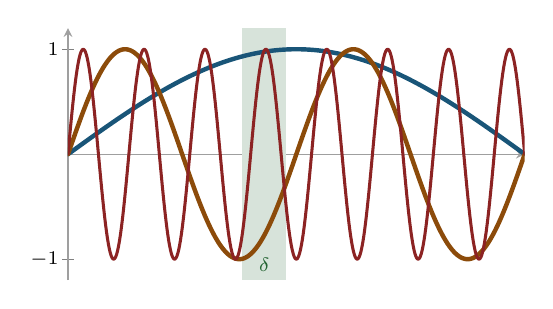
\begin{tikzpicture}
        \begin{axis}[
          axis background/.style={fill=white, fill opacity=0.6},
          scale only axis, width=5.8cm, height=3.2cm,
          xmin=0, xmax=3.1416, ymin=-1.2, ymax=1.2,
          axis x line=middle, axis y line=left, axis line style={gray!75},
          xtick=\empty, ytick={-1,1},
          tick label style={font=\scriptsize, fill=white, fill opacity=0.6, text opacity=1, inner sep=1pt},
          every axis plot/.append style={curveln},
        ]
          \fill[proofcolor!18] (axis cs:1.2,-1.2) rectangle (axis cs:1.5,1.2);
          \addplot[domain=0:3.1416, samples=150, defcolor] {sin(deg(x))};
          \addplot[domain=0:3.1416, samples=250, excolor] {sin(deg(4*x))};
          \addplot[domain=0:3.1416, samples=500, thmcolor, line width=1.1pt] {sin(deg(15*x))};
          \node[proofcolor, font=\scriptsize] at (axis cs:1.35,-1.05) {$\delta$};
        \end{axis}
      \end{tikzpicture}\\[0.2em]
      \hl{\small $\bigl|\sin n\tfrac{\pi}{2n} - \sin 0\bigr| = 1$ with distance $\tfrac{\pi}{2n} \to 0$}
    \end{column}
  \end{columns}

  \note{
    Two families illustrate the definition. In each panel the green
    vertical strip has the same width delta. On the left are shifted sine
    curves, sine of "x" plus "c", drawn in blue, brown, and red. Their
    slopes are at most 1, so within the strip each one changes by at most
    delta, and delta equal to epsilon works for all of them. On the right
    are sine of "n" "x" for "n" equal to 1, 4, and 15. The fast red wave
    swings from top to bottom inside the strip. The formula below shows
    why: the values at zero and at pi over 2 "n" differ by 1, while the
    distance tends to zero. No single delta works.
  }
\end{frame}

% --- Build 1/2 ---
\begin{frame}{Remarks on Equicontinuity}
  \begin{remblock}{Remark}
    Every member of an equicontinuous family is \alert{uniformly continuous}.
  \end{remblock}

  \note{
    Two quick remarks. First, if a family is equicontinuous, then each
    single member is uniformly continuous. That is immediate: the delta
    that works for the whole family works in particular for one function.
    So equicontinuity is a strengthening of uniform continuity.
  }
\end{frame}

% --- Build 2/2 ---
\begin{frame}{Remarks on Equicontinuity}
  \begin{remblock}{Remark}
    Every member of an equicontinuous family is \alert{uniformly continuous}.
  \end{remblock}

  \begin{remblock}{Remark}
    The sequence of Example 7.21 is \alert{not} equicontinuous:
    \[
      \Bigl| f_n\!\left(\tfrac1n\right) - f_n(0) \Bigr| = 1
      \quad\text{while}\quad d\!\left(\tfrac1n, 0\right) = \tfrac1n \to 0.
    \]
  \end{remblock}

  \note{
    Second, the moving spikes of Example 7.21 are not equicontinuous.
    Each "f" sub "n" equals 1 at the point one over "n" and 0 at the
    origin, so it climbs by 1 over a distance of only one over "n". For
    epsilon equal to 1, any proposed delta fails as soon as one over "n"
    is smaller than delta. This is exactly the behavior that prevented a
    uniformly convergent subsequence.
  }
\end{frame}

\begin{frame}{Where We Are Heading}
  \begin{hlbox}
  \begin{itemize}
    \item \textbf{Theorems 7.24, 7.25:} a close relation between
      \alert{equicontinuity} and \alert{uniform convergence} of sequences of
      continuous functions
    \item \textbf{But first, Theorem 7.23:} a selection process that has
      \emph{nothing to do with continuity}
  \end{itemize}
  \end{hlbox}

  \note{
    Rudin now announces the plan. Theorems 7.24 and 7.25 will show that
    equicontinuity and uniform convergence of continuous functions are
    closely tied together. But first we need a purely combinatorial tool,
    Theorem 7.23. It says nothing about continuity at all; it only uses
    boundedness at countably many points. It is the diagonal process
    promised earlier.
  }
\end{frame}
}

{
\usebackgroundtemplate{%
  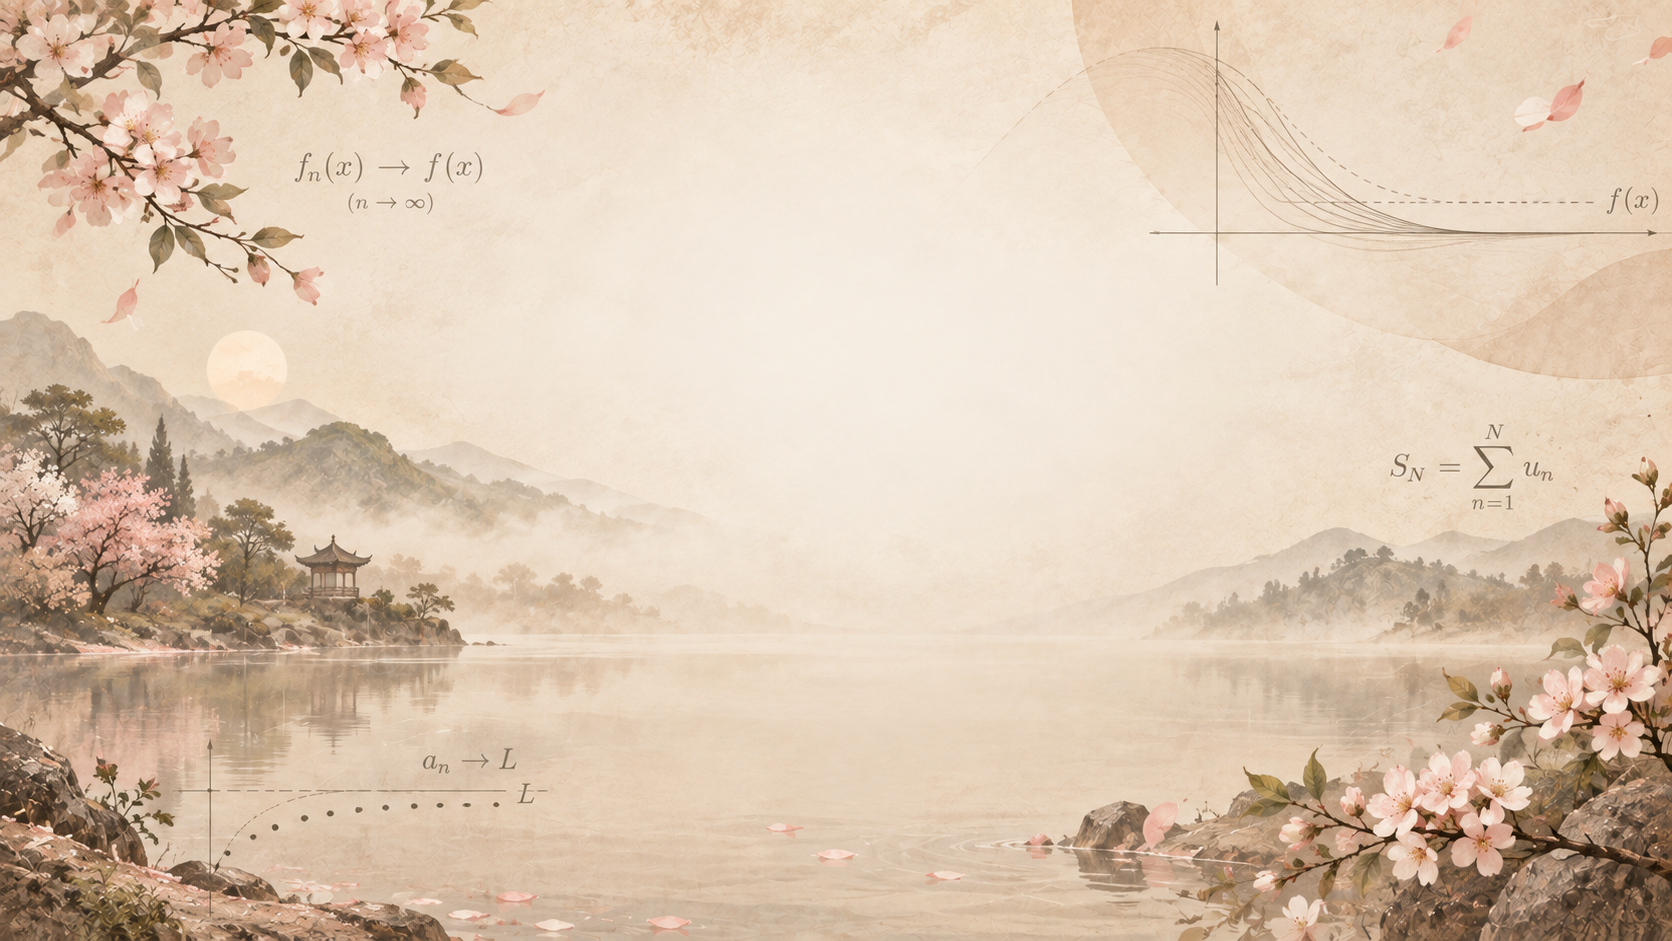
\includegraphics[width=\paperwidth,height=\paperheight,keepaspectratio=false]{chapter_07_bg_05.png}%
}
\section{The Diagonal Process}

\begin{frame}{Theorem 7.23: A Selection Theorem}
  \begin{thmblock}{Theorem 7.23}
    If $\{f_n\}$ is a \alert{pointwise bounded} sequence of complex functions
    on a \alert{countable} set $E$, then $\{f_n\}$ has a subsequence
    $\{f_{n_k}\}$ such that $\{f_{n_k}(x)\}$ converges for every $x \in E$.
  \end{thmblock}

  \vspace{0.4em}
  \begin{hlbox}
  \textbf{Strategy:}
  \begin{enumerate}
    \item Handle the points $x_1, x_2, x_3, \dots$ one at a time, passing to
      ever smaller subsequences $S_1, S_2, S_3, \dots$
    \item Take the \alert{diagonal} of the resulting array.
  \end{enumerate}
  \end{hlbox}

  \note{
    Here is the theorem. If the sequence is pointwise bounded on a
    countable set capital "E", then some subsequence converges at every
    point of capital "E". The strategy has two steps. We list the points
    of capital "E" as "x" sub 1, "x" sub 2, and so on, and handle them
    one at a time, each time passing to a smaller subsequence. No single
    one of these subsequences works for all points, so at the end we take
    the diagonal of the array they form.
  }
\end{frame}

\begin{frame}{Proof of Theorem 7.23 --- Step 1: The First Point}
  \begin{proofblock}{Step 1}
    Arrange the points of $E$ in a sequence $\{x_i\}$, $i = 1, 2, 3, \dots$

    \medskip
    $\{f_n(x_1)\}$ is a \alert{bounded} sequence of complex numbers, so by
    Theorem 3.6 it has a convergent subsequence:
    \[
      S_1\colon\; f_{1,1},\; f_{1,2},\; f_{1,3},\; \dots
      \qquad \text{with } \{f_{1,k}(x_1)\} \text{ convergent as } k \to \infty.
    \]
  \end{proofblock}

  \note{
    Since capital "E" is countable, we can arrange its points in a
    sequence. Start with the first point "x" sub 1. The numbers "f" sub
    "n" of "x" sub 1 form a bounded sequence of complex numbers, so by
    Theorem 3.6 some subsequence converges. We call this subsequence
    capital "S" sub 1, and write its terms with two indices: "f" sub 1
    comma "k". The first index records the stage, the second the position.
  }
\end{frame}

% --- Build 1/3 ---
\begin{frame}{Proof of Theorem 7.23 --- Step 2: The Array}
  \begin{center}
  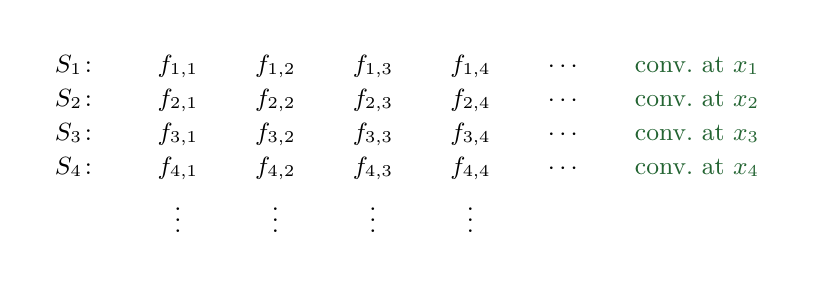
\begin{tikzpicture}[bgveil]
    \matrix (m) [matrix of math nodes, ampersand replacement=\&, column sep=0.55cm, row sep=-0.04cm,
      nodes={anchor=base, font=\small, inner sep=2.5pt}] {
      S_1\colon \& f_{1,1} \& f_{1,2} \& f_{1,3} \& f_{1,4} \& \cdots \& |[text=proofcolor]| \text{conv.\ at } x_1 \\
      S_2\colon \& f_{2,1} \& f_{2,2} \& f_{2,3} \& f_{2,4} \& \cdots \& |[text=proofcolor]| \text{conv.\ at } x_2 \\
      S_3\colon \& f_{3,1} \& f_{3,2} \& f_{3,3} \& f_{3,4} \& \cdots \& |[text=proofcolor]| \text{conv.\ at } x_3 \\
      S_4\colon \& f_{4,1} \& f_{4,2} \& f_{4,3} \& f_{4,4} \& \cdots \& |[text=proofcolor]| \text{conv.\ at } x_4 \\
      \& \vdots \& \vdots \& \vdots \& \vdots \& \& \\
    };
  \end{tikzpicture}
  \end{center}

  \vspace{-0.3em}
  \begin{proofblock}{Properties of the array}
    \begin{enumerate}
      \item[(a)] $S_n$ is a \alert{subsequence} of $S_{n-1}$, for $n = 2, 3, 4, \dots$
    \end{enumerate}
  \end{proofblock}

  \note{
    Now we repeat this step forever, producing sequences capital "S" sub
    1, capital "S" sub 2, capital "S" sub 3, and so on, arranged as rows
    of the array on the slide. Property "a" says that each row is a
    subsequence of the row above it. In other words, capital "S" sub 2
    is obtained by deleting some terms of capital "S" sub 1, capital "S"
    sub 3 by deleting some terms of capital "S" sub 2, and so on.
  }
\end{frame}

% --- Build 2/3 ---
\begin{frame}{Proof of Theorem 7.23 --- Step 2: The Array}
  \begin{center}
  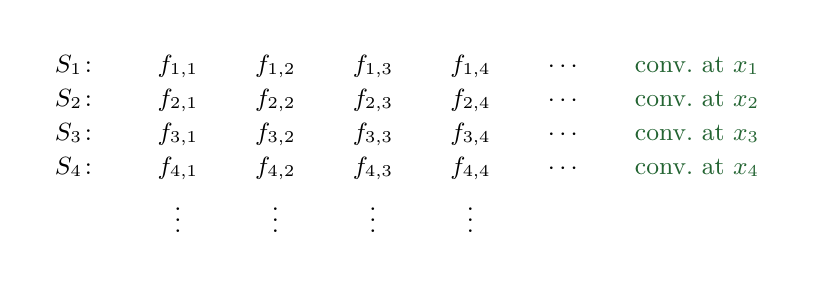
\begin{tikzpicture}[bgveil]
    \matrix (m) [matrix of math nodes, ampersand replacement=\&, column sep=0.55cm, row sep=-0.04cm,
      nodes={anchor=base, font=\small, inner sep=2.5pt}] {
      S_1\colon \& f_{1,1} \& f_{1,2} \& f_{1,3} \& f_{1,4} \& \cdots \& |[text=proofcolor]| \text{conv.\ at } x_1 \\
      S_2\colon \& f_{2,1} \& f_{2,2} \& f_{2,3} \& f_{2,4} \& \cdots \& |[text=proofcolor]| \text{conv.\ at } x_2 \\
      S_3\colon \& f_{3,1} \& f_{3,2} \& f_{3,3} \& f_{3,4} \& \cdots \& |[text=proofcolor]| \text{conv.\ at } x_3 \\
      S_4\colon \& f_{4,1} \& f_{4,2} \& f_{4,3} \& f_{4,4} \& \cdots \& |[text=proofcolor]| \text{conv.\ at } x_4 \\
      \& \vdots \& \vdots \& \vdots \& \vdots \& \& \\
    };
  \end{tikzpicture}
  \end{center}

  \vspace{-0.3em}
  \begin{proofblock}{Properties of the array}
    \begin{enumerate}
      \item[(a)] $S_n$ is a \alert{subsequence} of $S_{n-1}$, for $n = 2, 3, 4, \dots$
      \item[(b)] $\{f_{n,k}(x_n)\}$ \alert{converges} as $k \to \infty$
        (possible since $\{f_n(x_n)\}$ is bounded)
    \end{enumerate}
  \end{proofblock}

  \note{
    Property "b" says how each row is chosen. Row number "n" is a
    subsequence of the row above that converges at the point "x" sub
    "n". This is possible because the values at "x" sub "n" are bounded,
    so Theorem 3.6 applies again. The green labels at the right of the
    array record this. And since each row is a subsequence of all the
    rows above it, row number "n" in fact converges at all of the points
    "x" sub 1 through "x" sub "n".
  }
\end{frame}

% --- Build 3/3 ---
\begin{frame}{Proof of Theorem 7.23 --- Step 2: The Array}
  \begin{center}
  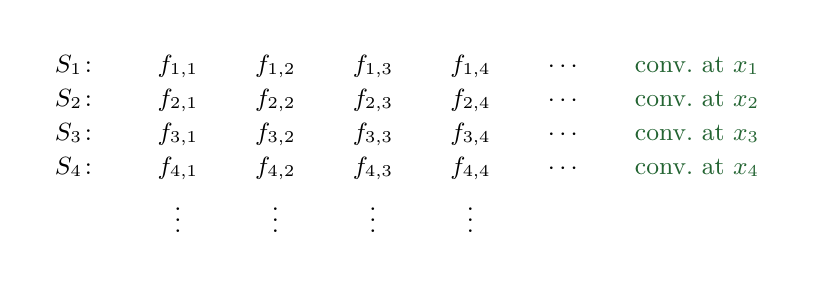
\begin{tikzpicture}[bgveil]
    \matrix (m) [matrix of math nodes, ampersand replacement=\&, column sep=0.55cm, row sep=-0.04cm,
      nodes={anchor=base, font=\small, inner sep=2.5pt}] {
      S_1\colon \& f_{1,1} \& f_{1,2} \& f_{1,3} \& f_{1,4} \& \cdots \& |[text=proofcolor]| \text{conv.\ at } x_1 \\
      S_2\colon \& f_{2,1} \& f_{2,2} \& f_{2,3} \& f_{2,4} \& \cdots \& |[text=proofcolor]| \text{conv.\ at } x_2 \\
      S_3\colon \& f_{3,1} \& f_{3,2} \& f_{3,3} \& f_{3,4} \& \cdots \& |[text=proofcolor]| \text{conv.\ at } x_3 \\
      S_4\colon \& f_{4,1} \& f_{4,2} \& f_{4,3} \& f_{4,4} \& \cdots \& |[text=proofcolor]| \text{conv.\ at } x_4 \\
      \& \vdots \& \vdots \& \vdots \& \vdots \& \& \\
    };
  \end{tikzpicture}
  \end{center}

  \vspace{-0.3em}
  \begin{proofblock}{Properties of the array}
    \begin{enumerate}
      \item[(a)] $S_n$ is a \alert{subsequence} of $S_{n-1}$, for $n = 2, 3, 4, \dots$
      \item[(b)] $\{f_{n,k}(x_n)\}$ \alert{converges} as $k \to \infty$
        (possible since $\{f_n(x_n)\}$ is bounded)
      \item[(c)] \alert{Order} is preserved: going down, functions move \emph{left}, never \emph{right}.
    \end{enumerate}
  \end{proofblock}

  \note{
    Property "c" is about order. Since each row is obtained by deleting
    terms, the surviving functions keep their original order. If one
    function comes before another in capital "S" sub 1, it still comes
    before it in every later row, as long as both survive. When terms are
    deleted, the remaining ones slide to the left to fill the gaps, but
    they never move to the right.
  }
\end{frame}

% --- Build 1/2 ---
\begin{frame}{Proof of Theorem 7.23 --- Step 3: Down the Diagonal}
  \begin{center}
  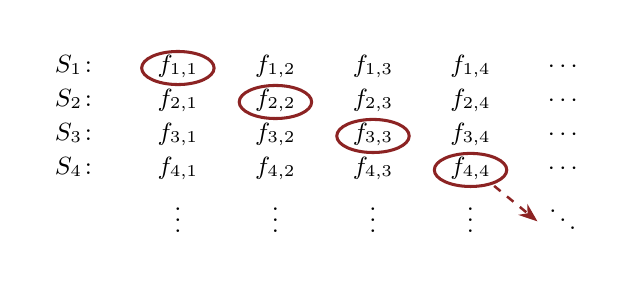
\begin{tikzpicture}[bgveil]
    \matrix (m) [matrix of math nodes, ampersand replacement=\&, column sep=0.55cm, row sep=-0.04cm,
      nodes={anchor=base, font=\small, inner sep=2.5pt}] {
      S_1\colon \& f_{1,1} \& f_{1,2} \& f_{1,3} \& f_{1,4} \& \cdots \\
      S_2\colon \& f_{2,1} \& f_{2,2} \& f_{2,3} \& f_{2,4} \& \cdots \\
      S_3\colon \& f_{3,1} \& f_{3,2} \& f_{3,3} \& f_{3,4} \& \cdots \\
      S_4\colon \& f_{4,1} \& f_{4,2} \& f_{4,3} \& f_{4,4} \& \cdots \\
      \& \vdots \& \vdots \& \vdots \& \vdots \& \ddots \\
    };
    \foreach \i/\j in {1/2, 2/3, 3/4, 4/5}
      \draw[thmcolor, line width=1.1pt] ([yshift=0.35ex]m-\i-\j.base) ellipse (0.46cm and 0.21cm);
    \draw[thmcolor, dashed, line width=0.9pt, -{Stealth[length=2.4mm]}]
      ([shift={(0.3,-0.15)}]m-4-5.base) -- ++(0.55,-0.45);
  \end{tikzpicture}
  \end{center}

  \vspace{-0.3em}
  \begin{proofblock}{The diagonal sequence}
    \[
      S\colon\quad f_{1,1},\; f_{2,2},\; f_{3,3},\; f_{4,4},\; \dots
    \]
  \end{proofblock}

  \note{
    Now we go down the diagonal of the array, circled in red, and the
    dashed arrow indicates that the pattern continues forever. The new
    sequence capital "S" takes the first term of the first row, the second
    term of the second row, the third term of the third row, and so on. By
    property "c", these terms appear in increasing order of the original
    sequence, so capital "S" really is a subsequence of "f" sub "n". The
    idea is that capital "S" eventually lives inside every row.
  }
\end{frame}

% --- Build 2/2 ---
\begin{frame}{Proof of Theorem 7.23 --- Step 3: Down the Diagonal}
  \begin{center}
  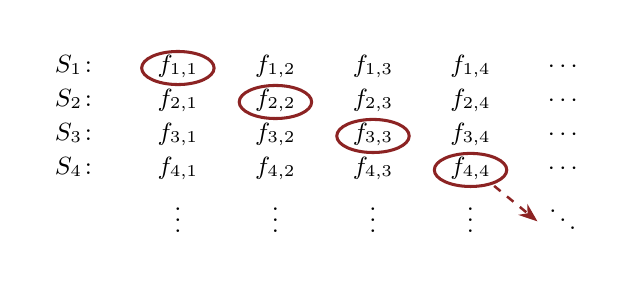
\begin{tikzpicture}[bgveil]
    \matrix (m) [matrix of math nodes, ampersand replacement=\&, column sep=0.55cm, row sep=-0.04cm,
      nodes={anchor=base, font=\small, inner sep=2.5pt}] {
      S_1\colon \& f_{1,1} \& f_{1,2} \& f_{1,3} \& f_{1,4} \& \cdots \\
      S_2\colon \& f_{2,1} \& f_{2,2} \& f_{2,3} \& f_{2,4} \& \cdots \\
      S_3\colon \& f_{3,1} \& f_{3,2} \& f_{3,3} \& f_{3,4} \& \cdots \\
      S_4\colon \& f_{4,1} \& f_{4,2} \& f_{4,3} \& f_{4,4} \& \cdots \\
      \& \vdots \& \vdots \& \vdots \& \vdots \& \ddots \\
    };
    \foreach \i/\j in {1/2, 2/3, 3/4, 4/5}
      \draw[thmcolor, line width=1.1pt] ([yshift=0.35ex]m-\i-\j.base) ellipse (0.46cm and 0.21cm);
    \draw[thmcolor, dashed, line width=0.9pt, -{Stealth[length=2.4mm]}]
      ([shift={(0.3,-0.15)}]m-4-5.base) -- ++(0.55,-0.45);
  \end{tikzpicture}
  \end{center}

  \vspace{-0.3em}
  \begin{proofblock}{The diagonal sequence}
    \[
      S\colon\quad f_{1,1},\; f_{2,2},\; f_{3,3},\; f_{4,4},\; \dots
    \]
    By (c), $S$ minus its first $n-1$ terms is a subsequence of $S_n$; by (b),
    $\{f_{n,n}(x_i)\}$ \alert{converges} for every $x_i \in E$. \hfill$\blacksquare$
  \end{proofblock}

  \note{
    Here is the conclusion. Fix a row number "n". From position "n" on,
    every diagonal term lies in row "n" or below, hence is a term of
    capital "S" sub "n", and by property "c" these terms appear in the
    right order. So, apart from its first "n" minus 1 terms, capital "S"
    is a subsequence of capital "S" sub "n". Since capital "S" sub "n"
    converges at "x" sub "n", so does capital "S". This holds for every
    "n", so the diagonal sequence converges at every point of capital
    "E".
  }
\end{frame}
}

{
\usebackgroundtemplate{%
  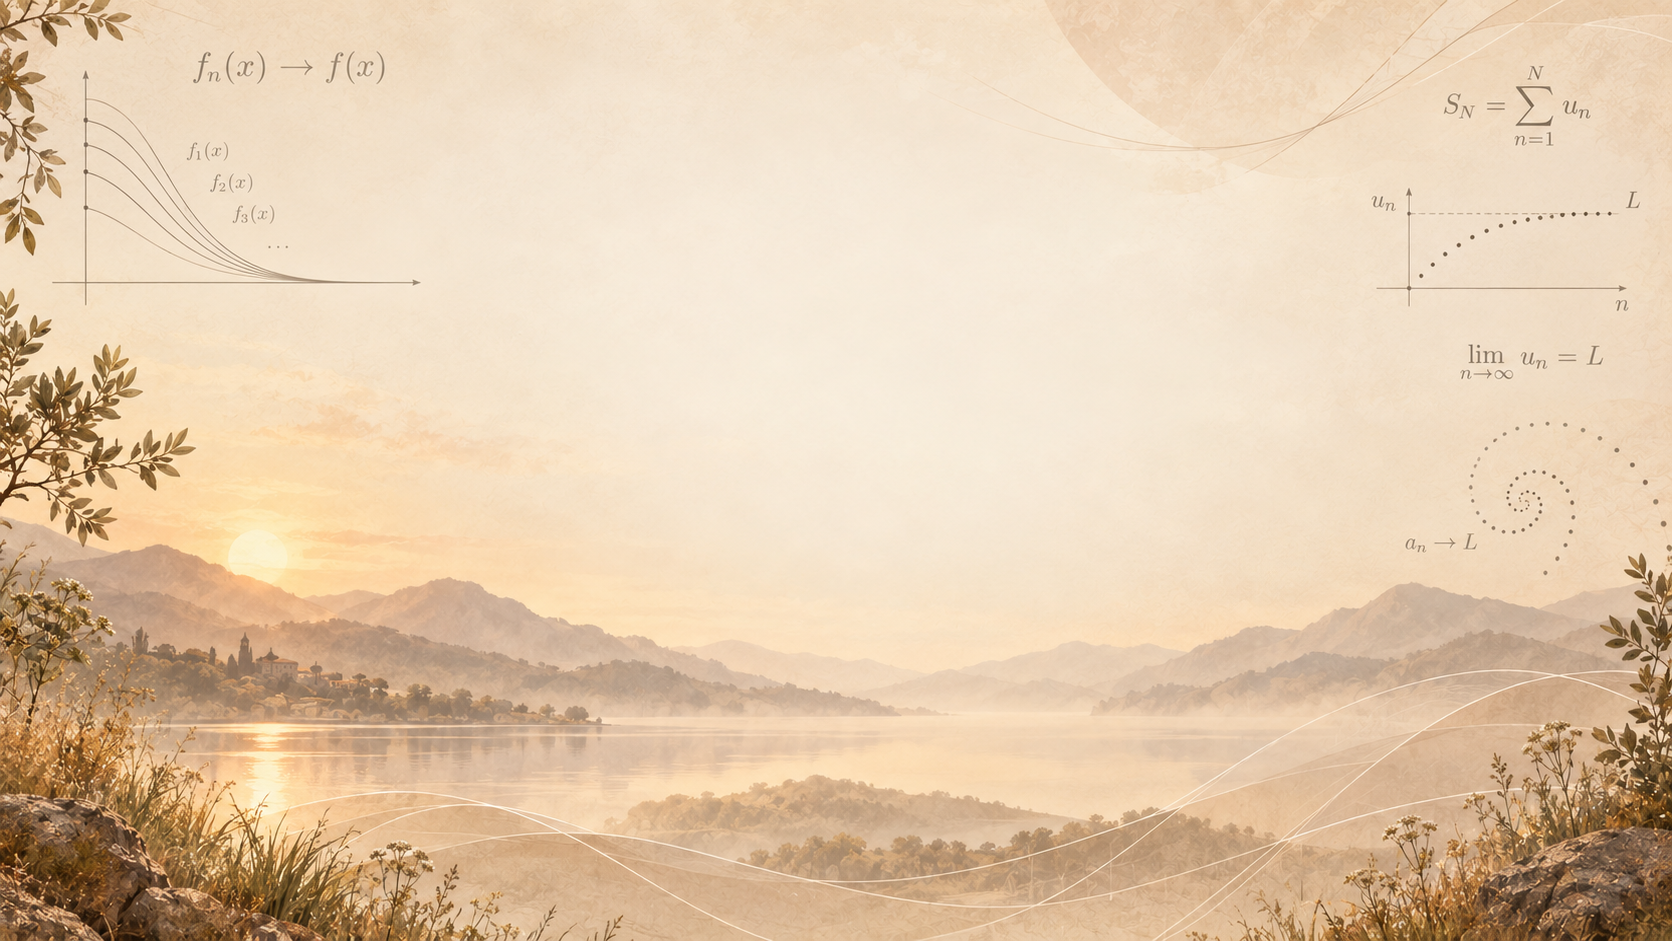
\includegraphics[width=\paperwidth,height=\paperheight,keepaspectratio=false]{chapter_07_bg_06.png}%
}
\section{Uniform Convergence Implies Equicontinuity}

\begin{frame}{Theorem 7.24}
  \begin{thmblock}{Theorem 7.24}
    If $K$ is a \alert{compact} metric space, if $f_n \in \mathscr{C}(K)$ for
    $n = 1, 2, 3, \dots$, and if $\{f_n\}$ \alert{converges uniformly} on $K$,
    then $\{f_n\}$ is \alert{equicontinuous} on $K$.
  \end{thmblock}

  \vspace{0.4em}
  \begin{hlbox}
  \textbf{Key idea:} for $n > N$, $f_n$ stays within $\varepsilon$ of the
  \emph{single} function $f_N$, and finitely many functions
  $f_1, \dots, f_N$ can share one $\delta$.
  \end{hlbox}

  \note{
    Our first link between the two concepts. Recall that script capital
    "C" of capital "K" is the space of continuous bounded complex
    functions on capital "K", from Definition 7.14. The theorem says that
    a uniformly convergent sequence of continuous functions on a compact
    space is automatically equicontinuous. The key idea is in the line
    below the box: the tail of the sequence hugs one function "f" sub
    capital "N", and the finitely many functions at the start can be
    handled together.
  }
\end{frame}

% --- Build 1/3 ---
\begin{frame}{Proof of Theorem 7.24}
  \begin{proofblock}{Step 1: Uniform convergence}
    Let $\varepsilon > 0$. Since $\{f_n\}$ converges uniformly, there is an integer
    $N$ with
    \[
      \|f_n - f_N\| < \varepsilon \qquad (n > N). \tag{42}
    \]
  \end{proofblock}

  \note{
    Let epsilon be positive. By the uniform Cauchy criterion, Theorem 7.8,
    uniform convergence gives an integer capital "N" such that every later
    function is within epsilon of "f" sub capital "N" in the supremum norm
    of Definition 7.14. This is equation 42. In words, beyond capital "N",
    every function lies in an epsilon tube around the graph of "f" sub
    capital "N".
  }
\end{frame}

% --- Build 2/3 ---
\begin{frame}{Proof of Theorem 7.24}
  \begin{proofblock}{Step 1: Uniform convergence}
    Let $\varepsilon > 0$. Since $\{f_n\}$ converges uniformly, there is an integer
    $N$ with
    \[
      \|f_n - f_N\| < \varepsilon \qquad (n > N). \tag{42}
    \]
  \end{proofblock}

  \begin{proofblock}{Step 2: Finitely many functions}
    Continuous functions on compact sets are \alert{uniformly continuous}, so
    there is a $\delta > 0$ with
    \[
      |f_i(x) - f_i(y)| < \varepsilon \quad \text{if } 1 \le i \le N,\; d(x, y) < \delta. \tag{43}
    \]
  \end{proofblock}

  \note{
    Next, each of the finitely many functions "f" sub 1 through "f" sub
    capital "N" is continuous on a compact space, hence uniformly
    continuous by Theorem 4.19. Each one gives its own delta, and we take
    the smallest of these finitely many deltas. This single delta works
    for all of them, as equation 43 says. Finiteness is essential here:
    the minimum of infinitely many positive numbers could be zero.
  }
\end{frame}

% --- Build 3/3 ---
\begin{frame}{Proof of Theorem 7.24}
  \begin{proofblock}{So far}
    $\|f_n - f_N\| < \varepsilon$ for $n > N$ \hfill (42)\\
    $|f_i(x) - f_i(y)| < \varepsilon$ if $1 \le i \le N$, $d(x, y) < \delta$ \hfill (43)
  \end{proofblock}

  \begin{proofblock}{Step 3: The tail, via the triangle inequality}
    If $n > N$ and $d(x, y) < \delta$:
    \[
      |f_n(x) - f_n(y)| \le
      \underbrace{|f_n(x) - f_N(x)|}_{< \varepsilon \text{ by (42)}}
      + \underbrace{|f_N(x) - f_N(y)|}_{< \varepsilon \text{ by (43)}}
      + \underbrace{|f_N(y) - f_n(y)|}_{< \varepsilon \text{ by (42)}}
      < \alert{3\varepsilon}.
    \]
    With (43), this holds for \emph{all} $n$. \hfill$\blacksquare$
  \end{proofblock}

  \note{
    The box at the top recalls equations 42 and 43. Now take any "n"
    beyond capital "N" and two points within delta.
    We go from "f" sub "n" of "x" to "f" sub capital "N" of "x", then
    across to "f" sub capital "N" of "y", and then back to "f" sub "n" of
    "y". The first and last jumps are small by equation 42, the middle one
    by equation 43, so the total is less than 3 epsilon. Together with
    equation 43 for the first capital "N" functions, one delta works for
    the whole sequence, which is equicontinuity.
  }
\end{frame}

\begin{frame}{The $3\varepsilon$ Argument in a Picture}
  \tikzset{segnum/.style={circle, draw=proofcolor, line width=0.9pt, fill=white, text=proofcolor, font=\small\bfseries, inner sep=1.2pt, minimum size=1.3em}}
  \begin{center}
  \begin{tikzpicture}
    \begin{axis}[
      axis background/.style={fill=white, fill opacity=0.6},
      scale only axis, width=10.5cm, height=4.6cm,
      xmin=0, xmax=4, ymin=-0.2, ymax=1.8,
      axis x line=bottom, axis y line=left, axis line style={gray!75},
      xtick={1.4,2.1}, xticklabels={$x$,$y$}, ytick=\empty,
      tick label style={font=\small, fill=white, fill opacity=0.6, text opacity=1, inner sep=1pt},
      every axis plot/.append style={curveln},
    ]
      \addplot[name path=up, draw=none, domain=0:4, samples=100] {0.6*sin(deg(x)) + 0.2*x + 0.35};
      \addplot[name path=lo, draw=none, domain=0:4, samples=100] {0.6*sin(deg(x)) + 0.2*x - 0.35};
      \addplot[defcolor!15] fill between[of=up and lo];
      \addplot[domain=0:4, samples=150, defcolor] {0.6*sin(deg(x)) + 0.2*x};
      \addplot[domain=0:4, samples=250, thmcolor] {0.6*sin(deg(x)) + 0.2*x + 0.25*sin(deg(5*x))};
      \draw[gray, projln] (axis cs:1.4,-0.2) -- (axis cs:1.4,1.8);
      \draw[gray, projln] (axis cs:2.1,-0.2) -- (axis cs:2.1,1.8);
      \draw[proofcolor, line width=1.6pt] (axis cs:1.4,1.0355) -- (axis cs:1.4,0.8713);
      \draw[proofcolor, line width=1.6pt] (axis cs:1.4,0.8713) -- (axis cs:2.1,0.9379);
      \draw[proofcolor, line width=1.6pt] (axis cs:2.1,0.9379) -- (axis cs:2.1,0.7180);
      \node[segnum] at (axis cs:1.2,1.13) {1};
      \node[segnum] at (axis cs:1.75,0.68) {2};
      \node[segnum] at (axis cs:2.1,0.47) {3};
      \dotpt{thmcolor}{(axis cs:1.4,1.0355)}
      \dotpt{defcolor}{(axis cs:1.4,0.8713)}
      \dotpt{defcolor}{(axis cs:2.1,0.9379)}
      \dotpt{thmcolor}{(axis cs:2.1,0.7180)}
      \node[defcolor, font=\small, anchor=west] at (axis cs:3.35,1.15) {$f_N$};
      \node[thmcolor, font=\small, anchor=west] at (axis cs:3.45,0.55) {$f_n$};
      \node[defcolor, font=\scriptsize] at (axis cs:0.45,0.75) {$\varepsilon$-tube};
    \end{axis}
  \end{tikzpicture}
  \end{center}

  \note{
    Here is the argument as a picture. The blue curve is "f" sub capital
    "N", and the light blue band around it is the epsilon tube from
    equation 42. The red curve is a later function "f" sub "n", which
    stays inside the tube. The dashed vertical lines mark two nearby
    points "x" and "y". The green path has three pieces, marked by the
    circled numbers 1, 2, and 3. Piece 1 drops from the red curve to the
    blue curve at "x", and it is short because the red curve stays in the
    tube. Piece 2 joins the two blue points, and it is short because "f"
    sub capital "N" is uniformly continuous, by equation 43. Piece 3 goes
    from the blue curve back down to the red one at "y", short again
    because of the tube. Three pieces, each shorter than epsilon, give the
    bound 3 epsilon.
  }
\end{frame}
}

{
\usebackgroundtemplate{%
  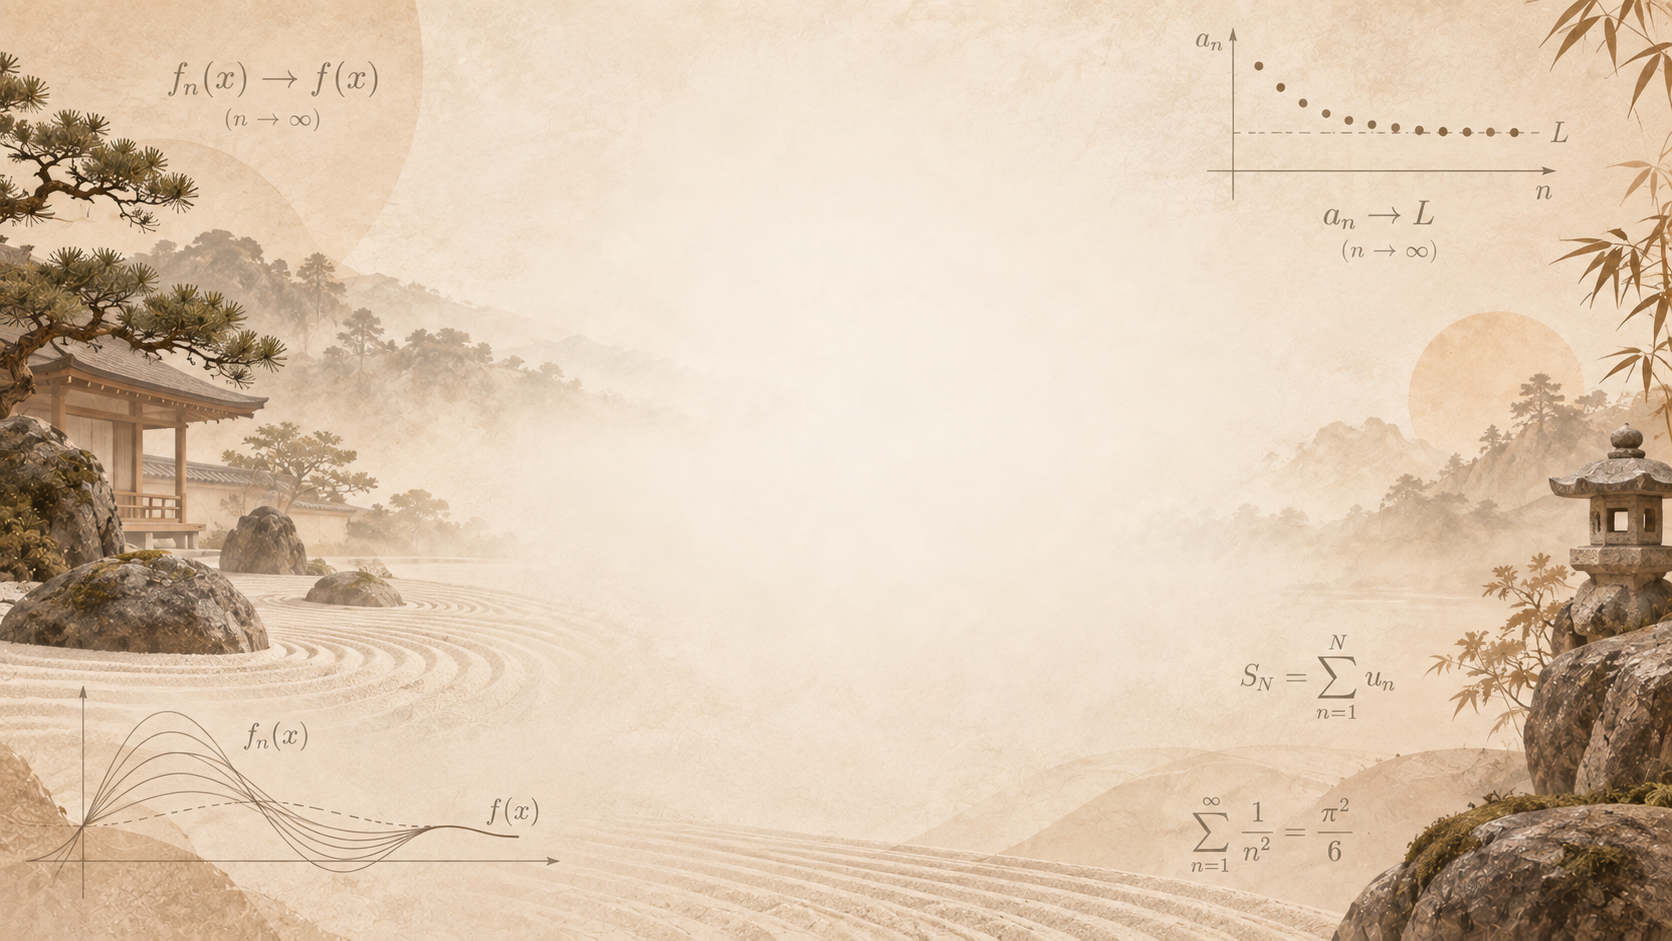
\includegraphics[width=\paperwidth,height=\paperheight,keepaspectratio=false]{chapter_07_bg_07.png}%
}
\section{The Main Theorem}

\begin{frame}{Theorem 7.25: Uniformly Convergent Subsequences}
  \begin{thmblock}{Theorem 7.25 (Arzel\`a--Ascoli)}
    If $K$ is \alert{compact}, if $f_n \in \mathscr{C}(K)$ for $n = 1, 2, 3, \dots$,
    and if $\{f_n\}$ is \alert{pointwise bounded} and \alert{equicontinuous}
    on $K$, then
    \begin{enumerate}
      \item[(a)] $\{f_n\}$ is uniformly bounded on $K$,
      \item[(b)] $\{f_n\}$ contains a \alert{uniformly convergent subsequence}.
    \end{enumerate}
  \end{thmblock}

  \vspace{0.3em}
  \begin{hlbox}
  \textbf{Compare:} Theorem 3.6 --- bounded sequences in $\mathbb{R}^k$ have
  convergent subsequences.
  \end{hlbox}

  \note{
    Here is the main theorem of the section, usually called the Arzela
    Ascoli theorem. Let capital "K" be compact, and let the "f" sub "n" be
    continuous on capital "K", pointwise bounded, and equicontinuous.
    Then part "a" says the sequence is automatically uniformly bounded,
    and part "b" says it has a uniformly convergent subsequence. This is
    the function version of Theorem 3.6, with equicontinuity as the extra
    ingredient that rules out the bad behavior of our two examples.
  }
\end{frame}

% --- Build 1/3 ---
\begin{frame}{Proof of Theorem 7.25(a): Uniform Boundedness}
  \begin{columns}[T]
    \begin{column}{0.56\textwidth}
      \begin{proofblock}{Step 1: Equicontinuity}
        Let $\varepsilon > 0$; by Definition 7.22 choose $\delta > 0$ with
        \[
          |f_n(x) - f_n(y)| < \varepsilon \tag{44}
        \]
        for all $n$, whenever $d(x, y) < \delta$.
      \end{proofblock}
    \end{column}
    \begin{column}{0.42\textwidth}
      \centering
      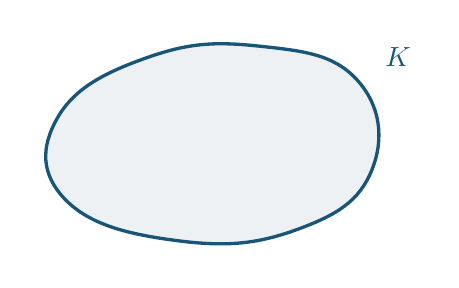
\begin{tikzpicture}[bgveil, scale=0.95]
        \Kblob
      \end{tikzpicture}
    \end{column}
  \end{columns}

  \note{
    Let's prove part "a". Fix a positive epsilon and use equicontinuity
    to choose delta, so that every function in the sequence changes by
    less than epsilon between any two points closer than delta. This is
    equation 44. The blue region on the right represents the compact
    space capital "K". Next, we use compactness to reduce the problem to
    finitely many points.
  }
\end{frame}

% --- Build 2/3 ---
\begin{frame}{Proof of Theorem 7.25(a): Uniform Boundedness}
  \begin{columns}[T]
    \begin{column}{0.56\textwidth}
      \begin{proofblock}{Step 1: Equicontinuity}
        Let $\varepsilon > 0$; by Definition 7.22 choose $\delta > 0$ with
        \[
          |f_n(x) - f_n(y)| < \varepsilon \tag{44}
        \]
        for all $n$, whenever $d(x, y) < \delta$.
      \end{proofblock}
      \begin{proofblock}{Step 2: Compactness}
        There are finitely many $p_1, \dots, p_r \in K$ such that every
        $x \in K$ has $d(x, p_i) < \delta$ for some $i$.
      \end{proofblock}
    \end{column}
    \begin{column}{0.42\textwidth}
      \centering
      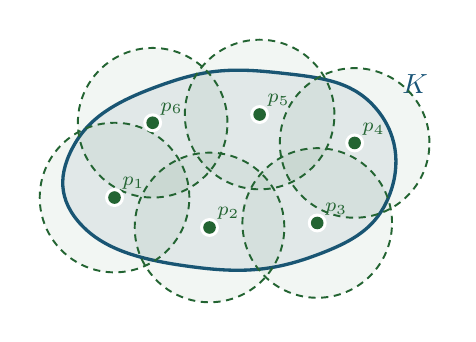
\begin{tikzpicture}[bgveil, scale=0.95]
        \Kblob
        \foreach \p in {(0.23,0.58), (1.5,0.18), (2.94,0.24), (3.44,1.31), (2.17,1.69), (0.74,1.58)}
          \draw[proofcolor, projln, fill=proofcolor, fill opacity=0.06] \p circle (1.0);
        \foreach \p/\l in {(0.23,0.58)/1, (1.5,0.18)/2, (2.94,0.24)/3, (3.44,1.31)/4, (2.17,1.69)/5, (0.74,1.58)/6}
          {\dotpt{proofcolor}{\p} \node[proofcolor, font=\scriptsize, above right=-1pt] at \p {$p_{\l}$};}
      \end{tikzpicture}\\[0.2em]
      \hl{\scriptsize balls of radius $\delta$ cover $K$}
    \end{column}
  \end{columns}

  \note{
    The open balls of radius delta, one around each point of capital "K",
    cover capital "K". By compactness, finitely many of them suffice. Their
    centers are the points "p" sub 1 through "p" sub "r". In the picture
    there are six of them, drawn as green dots, and the dashed green
    circles around them are the balls of radius delta that together
    cover the blue region. Every point of capital "K" is within delta of
    some "p" sub "i".
  }
\end{frame}

% --- Build 3/3 ---
\begin{frame}{Proof of Theorem 7.25(a): Uniform Boundedness}
  \begin{columns}[T]
    \begin{column}{0.56\textwidth}
      \begin{proofblock}{Step 2: Compactness}
        There are finitely many $p_1, \dots, p_r \in K$ such that every
        $x \in K$ has $d(x, p_i) < \delta$ for some $i$.
      \end{proofblock}
      \begin{proofblock}{Step 3: Pointwise bounds at $p_i$}
        Pointwise bounded: $|f_n(p_i)| < M_i\ \forall n$.\\
        Let $M = \max(M_1, \dots, M_r)$. Then
        \[
          |f_n(x)| \le |f_n(p_i)| + |f_n(x) - f_n(p_i)| < \alert{M + \varepsilon}.
        \]
        \vspace{-1.2em}\hfill$\blacksquare$
      \end{proofblock}
    \end{column}
    \begin{column}{0.42\textwidth}
      \centering
      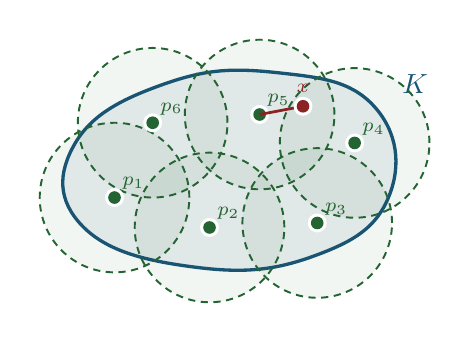
\begin{tikzpicture}[bgveil, scale=0.95]
        \Kblob
        \foreach \p in {(0.23,0.58), (1.5,0.18), (2.94,0.24), (3.44,1.31), (2.17,1.69), (0.74,1.58)}
          \draw[proofcolor, projln, fill=proofcolor, fill opacity=0.06] \p circle (1.0);
        \foreach \p/\l in {(0.23,0.58)/1, (1.5,0.18)/2, (2.94,0.24)/3, (3.44,1.31)/4, (2.17,1.69)/5, (0.74,1.58)/6}
          {\dotpt{proofcolor}{\p} \node[proofcolor, font=\scriptsize, above right=-1pt] at \p {$p_{\l}$};}
        \draw[thmcolor, line width=1pt] (2.75,1.8) -- (2.17,1.69);
        \dotpt{thmcolor}{(2.75,1.8)}
        \node[thmcolor, font=\scriptsize, above] at (2.75,1.85) {$x$};
      \end{tikzpicture}\\[0.2em]
      \hl{\scriptsize $x$ is within $\delta$ of some $p_i$}
    \end{column}
  \end{columns}

  \note{
    Now we use pointwise boundedness, but only at the finitely many
    centers. At each "p" sub "i" there is a bound capital "M" sub "i" for
    all the functions, and we let capital "M" be the largest of these
    finitely many bounds. Take any point "x", shown in red, and a center
    within delta of it. The value at "x" is at most the value at the
    center, which is below capital "M", plus the change from the center
    to "x", which is below epsilon by equation 44. So capital "M" plus
    epsilon is a uniform bound.
  }
\end{frame}

\begin{frame}{Proof Strategy: Theorem 7.25(b)}
  \begin{hlbox}
  \textbf{Goal:} a subsequence $\{g_i\}$ of $\{f_n\}$ that converges
  \alert{uniformly} on $K$.

  \vspace{0.6em}
  \textbf{Approach:}
  \begin{enumerate}
    \item Take a \alert{countable dense} subset $E \subset K$.
    \item Theorem 7.23: get $\{g_i\}$ converging at every point of $E$.
    \item Compactness: \alert{finitely many} points $x_1, \dots, x_m \in E$\\
      are $\delta$-close to all of $K$.
    \item Equicontinuity: closeness at $x_s$ spreads to nearby $x$.
    \item Show $\{g_i\}$ is \alert{uniformly Cauchy} ($3\varepsilon$ argument).
  \end{enumerate}
  \end{hlbox}

  \note{
    Before the details of part "b", here is the plan. We cannot control
    all points of capital "K" at once, so we start with a countable dense
    subset capital "E". The diagonal process of Theorem 7.23 gives a
    subsequence converging on capital "E". Compactness then lets us pick
    finitely many points of capital "E" that are close to everything.
    Equicontinuity transfers convergence at those points to every nearby
    point, and a 3 epsilon argument shows the subsequence is uniformly
    Cauchy.
  }
\end{frame}

% --- Build 1/2 ---
\begin{frame}{Proof of Theorem 7.25(b) --- Setup}
  \begin{columns}[T]
    \begin{column}{0.56\textwidth}
      \begin{proofblock}{Step 1: A countable dense set}
        Let $E \subset K$ be \alert{countable} and \alert{dense}
        (Exercise 25, Chapter 2). By Theorem 7.23, some subsequence
        $\{f_{n_i}\} =: \{g_i\}$ has $\{g_i(x)\}$ convergent for every
        $x \in E$.
      \end{proofblock}
    \end{column}
    \begin{column}{0.42\textwidth}
      \centering
      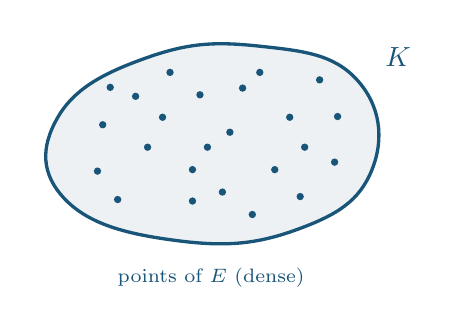
\begin{tikzpicture}[bgveil, scale=0.95]
        \Kblob
        \foreach \p in {(0.23,0.58),(0.5,0.2),(0.9,0.9),(1.5,0.18),(1.5,0.6),(1.9,0.3),(2.3,0.0),(2.6,0.6),(2.94,0.24),(3.4,0.7),(3.44,1.31),(3.2,1.8),(2.8,1.3),(2.4,1.9),(2.0,1.1),(1.6,1.6),(1.2,1.9),(0.74,1.58),(0.3,1.2),(1.1,1.3),(2.17,1.69),(3.0,0.9),(1.7,0.9),(0.4,1.7)}
          \fill[defcolor] \p circle (1.4pt);
        \node[defcolor, font=\scriptsize] at (1.75,-0.85) {points of $E$ (dense)};
      \end{tikzpicture}
    \end{column}
  \end{columns}

  \note{
    Step 1. Every compact metric space has a countable dense subset;
    this is Exercise 25 of Chapter 2. Call it capital "E". The small blue
    dots in the picture suggest such a set, spread throughout capital
    "K". Since capital "E" is countable and the sequence is pointwise
    bounded, Theorem 7.23 gives a subsequence that converges at every
    point of capital "E". To simplify notation we rename this
    subsequence "g" sub "i". We will show it converges uniformly on
    all of capital "K".
  }
\end{frame}

% --- Build 2/2 ---
\begin{frame}{Proof of Theorem 7.25(b) --- Setup}
  \begin{columns}[T]
    \begin{column}{0.56\textwidth}
      \begin{proofblock}{Step 1: A countable dense set}
        Let $E \subset K$ be \alert{countable} and \alert{dense}
        (Exercise 25, Chapter 2). By Theorem 7.23, some subsequence
        $\{f_{n_i}\} =: \{g_i\}$ has $\{g_i(x)\}$ convergent for every
        $x \in E$.
      \end{proofblock}
      \begin{proofblock}{Step 2: Finitely many centers in $E$}
        Fix $\varepsilon > 0$ and $\delta$ as in (44). Let
        $V(x, \delta) = \{y \in K : d(x, y) < \delta\}$. Then
        \[
          K \subset V(x_1, \delta) \cup \cdots \cup V(x_m, \delta) \tag{45}
        \]
        for some $x_1, \dots, x_m \in E$.
      \end{proofblock}
    \end{column}
    \begin{column}{0.42\textwidth}
      \centering
      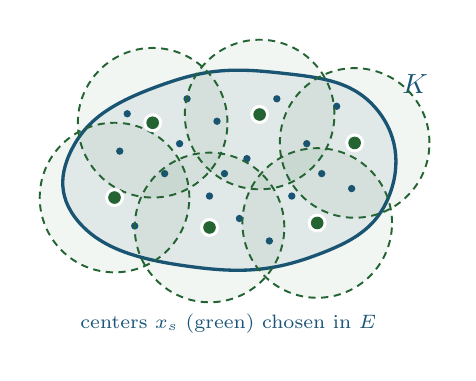
\begin{tikzpicture}[bgveil, scale=0.95]
        \Kblob
        \foreach \p in {(0.23,0.58),(0.5,0.2),(0.9,0.9),(1.5,0.18),(1.5,0.6),(1.9,0.3),(2.3,0.0),(2.6,0.6),(2.94,0.24),(3.4,0.7),(3.44,1.31),(3.2,1.8),(2.8,1.3),(2.4,1.9),(2.0,1.1),(1.6,1.6),(1.2,1.9),(0.74,1.58),(0.3,1.2),(1.1,1.3),(2.17,1.69),(3.0,0.9),(1.7,0.9),(0.4,1.7)}
          \fill[defcolor] \p circle (1.4pt);
        \foreach \p in {(0.23,0.58), (1.5,0.18), (2.94,0.24), (3.44,1.31), (2.17,1.69), (0.74,1.58)}
          \draw[proofcolor, projln, fill=proofcolor, fill opacity=0.06] \p circle (1.0);
        \foreach \p in {(0.23,0.58), (1.5,0.18), (2.94,0.24), (3.44,1.31), (2.17,1.69), (0.74,1.58)}
          {\dotpt{proofcolor}{\p}}
        \node[defcolor, font=\scriptsize] at (1.75,-1.1) {centers $x_s$ (green) chosen in $E$};
      \end{tikzpicture}
    \end{column}
  \end{columns}

  \note{
    Step 2. Fix epsilon and the delta from equation 44. Write capital
    "V" of "x" comma delta for the ball of radius delta around "x". Since
    capital "E" is dense, every point of capital "K" is within delta of
    some point of capital "E", so the balls centered at points of capital
    "E" cover capital "K". By compactness, finitely many suffice, with
    centers "x" sub 1 through "x" sub "m". That is equation 45. In the
    picture, the green dots are these centers, and the dashed green
    circles cover the blue region.
  }
\end{frame}

% --- Build 1/3 ---
\begin{frame}{Proof of Theorem 7.25(b) --- The $3\varepsilon$ Estimate}
  \begin{proofblock}{Step 3: Convergence at finitely many points}
    $\{g_i(x_s)\}$ converges for each of the finitely many $x_s \in E$, so there is
    $N$ with
    \[
      |g_i(x_s) - g_j(x_s)| < \varepsilon
      \quad \text{whenever } i \ge N,\; j \ge N,\; 1 \le s \le m. \tag{46}
    \]
  \end{proofblock}

  \note{
    Step 3. At each of the finitely many centers "x" sub "s", the
    sequence "g" sub "i" of "x" sub "s" converges, so it is a Cauchy
    sequence of numbers. Each center gives its own threshold, and we take
    capital "N" to be the largest of these finitely many thresholds. Then
    equation 46 holds for all centers at once. Once again, finiteness is
    what makes this maximum possible.
  }
\end{frame}

% --- Build 2/3 ---
\begin{frame}{Proof of Theorem 7.25(b) --- The $3\varepsilon$ Estimate}
  \begin{proofblock}{Step 3: Convergence at finitely many points}
    $\{g_i(x_s)\}$ converges for each of the finitely many $x_s \in E$, so there is
    $N$ with
    \[
      |g_i(x_s) - g_j(x_s)| < \varepsilon
      \quad \text{whenever } i \ge N,\; j \ge N,\; 1 \le s \le m. \tag{46}
    \]
  \end{proofblock}

  \begin{proofblock}{Step 4: Spread to every $x \in K$}
    For $x \in K$, (45) gives $x \in V(x_s, \delta)$ for some $s$, so by (44)
    \[
      |g_i(x) - g_i(x_s)| < \varepsilon \quad \text{for every } i.
    \]
  \end{proofblock}

  \note{
    Step 4. Now take an arbitrary point "x" of capital "K". By equation
    45, it lies in one of the balls, say the ball around "x" sub "s". The
    distance from "x" to "x" sub "s" is less than delta, so by
    equicontinuity, equation 44, every "g" sub "i" changes by less than
    epsilon between "x" and "x" sub "s". The same delta works for every
    "i", and that is exactly where equicontinuity is used.
  }
\end{frame}

% --- Build 3/3 ---
\begin{frame}{Proof of Theorem 7.25(b) --- The $3\varepsilon$ Estimate}
  \begin{hlbox}
  \textbf{So far:} $|g_i(x_s) - g_j(x_s)| < \varepsilon$ for $i, j \ge N$, $1 \le s \le m$ \hfill (46)
  \end{hlbox}

  \begin{proofblock}{Step 4: Spread to every $x \in K$}
    For $x \in K$, (45) gives $x \in V(x_s, \delta)$ for some $s$, so by (44)
    \[
      |g_i(x) - g_i(x_s)| < \varepsilon \quad \text{for every } i.
    \]
  \end{proofblock}

  \begin{proofblock}{Step 5: Uniformly Cauchy}
    If $i \ge N$ and $j \ge N$, then by (46):
    \[
      |g_i(x) - g_j(x)| \le |g_i(x) - g_i(x_s)| + |g_i(x_s) - g_j(x_s)| + |g_j(x_s) - g_j(x)|
      < \alert{3\varepsilon}.
    \]
    $N$ does not depend on $x$, so $\{g_i\}$ converges \alert{uniformly}
    (Theorem 7.8). \hfill$\blacksquare$
  \end{proofblock}

  \note{
    The line at the top recalls equation 46. Step 5 is the familiar 3
    epsilon argument. For "i" and "j" at least
    capital "N", go from "g" sub "i" of "x" to "g" sub "i" of "x" sub "s",
    then to "g" sub "j" of "x" sub "s", then back to "g" sub "j" of "x".
    The outer two pieces are small by step 4, the middle one by equation
    46. Since capital "N" was chosen without reference to "x", this is the
    uniform Cauchy criterion of Theorem 7.8, and the subsequence
    converges uniformly. This completes the proof.
  }
\end{frame}
}

{
\usebackgroundtemplate{%
  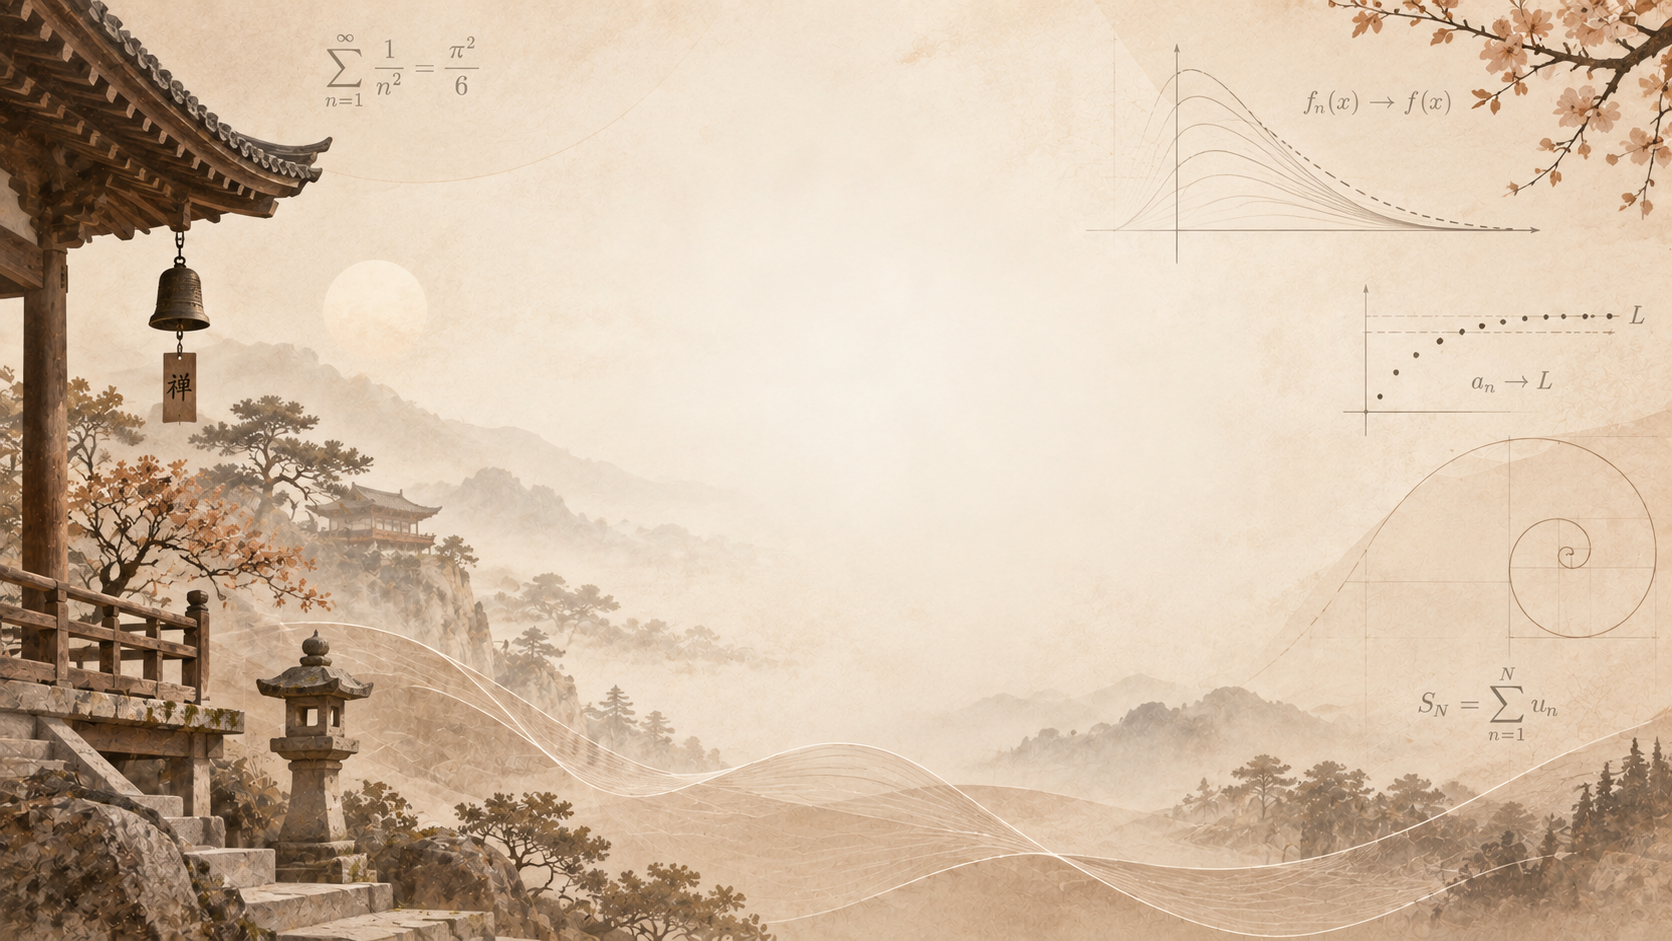
\includegraphics[width=\paperwidth,height=\paperheight,keepaspectratio=false]{chapter_07_bg_08.png}%
}
\section{Summary}

% --- Build 1/5 ---
\begin{frame}{Summary}
  \begin{hlbox}
  \small
  \textbf{Key takeaways from this section:}
  \begin{itemize}
    \item \textbf{Definition 7.19:} \alert{pointwise} vs.\ \alert{uniform}
      boundedness of $\{f_n\}$
  \end{itemize}
  \end{hlbox}

  \note{
    Let's review. We began with two notions of boundedness for a
    sequence of functions: pointwise bounded, where the bound may depend
    on the point, and uniformly bounded, where one constant works
    everywhere. Uniform boundedness is the stronger of the two, and the
    functions "f" sub "n" equal to the minimum of "n" and one over "x"
    showed that it really is stronger.
  }
\end{frame}

% --- Build 2/5 ---
\begin{frame}{Summary}
  \begin{hlbox}
  \small
  \textbf{Key takeaways from this section:}
  \begin{itemize}
    \item \textbf{Definition 7.19:} \alert{pointwise} vs.\ \alert{uniform}
      boundedness of $\{f_n\}$
    \item \textbf{Examples 7.20, 7.21:} boundedness is \alert{not enough}
      ($\sin nx$; moving spikes)
  \end{itemize}
  \end{hlbox}

  \note{
    Two examples showed that boundedness alone does not give the
    analogue of Theorem 3.6. The functions sine of "n" "x" have no
    subsequence converging at every point, and the moving spikes of
    Example 7.21 converge pointwise to zero but have no uniformly
    convergent subsequence.
  }
\end{frame}

% --- Build 3/5 ---
\begin{frame}{Summary}
  \begin{hlbox}
  \small
  \textbf{Key takeaways from this section:}
  \begin{itemize}
    \item \textbf{Definition 7.19:} \alert{pointwise} vs.\ \alert{uniform}
      boundedness of $\{f_n\}$
    \item \textbf{Examples 7.20, 7.21:} boundedness is \alert{not enough}
      ($\sin nx$; moving spikes)
    \item \textbf{Definition 7.22:} \alert{equicontinuity}: one $\delta$ for
      the whole family
  \end{itemize}
  \end{hlbox}

  \note{
    The missing ingredient was equicontinuity. Uniform continuity asks
    for one delta per function; equicontinuity asks for one delta that
    works for every function in the family at once. The moving spikes
    fail this test, which is exactly why they misbehave.
  }
\end{frame}

% --- Build 4/5 ---
\begin{frame}{Summary}
  \begin{hlbox}
  \small
  \textbf{Key takeaways from this section:}
  \begin{itemize}
    \item \textbf{Definition 7.19:} \alert{pointwise} vs.\ \alert{uniform}
      boundedness of $\{f_n\}$
    \item \textbf{Examples 7.20, 7.21:} boundedness is \alert{not enough}
      ($\sin nx$; moving spikes)
    \item \textbf{Definition 7.22:} \alert{equicontinuity}: one $\delta$ for
      the whole family
    \item \textbf{Theorem 7.23:} the \alert{diagonal process} handles countably
      many points
  \end{itemize}
  \end{hlbox}

  \note{
    Our main tool was the diagonal process of Theorem 7.23. By passing
    to smaller and smaller subsequences, one point at a time, and then
    reading off the diagonal, we turned convergence at each point
    separately into convergence at countably many points at once. No
    continuity was needed for this step.
  }
\end{frame}

% --- Build 5/5 ---
\begin{frame}{Summary}
  \begin{hlbox}
  \small
  \textbf{Key takeaways from this section:}
  \begin{itemize}
    \item \textbf{Definition 7.19:} \alert{pointwise} vs.\ \alert{uniform}
      boundedness of $\{f_n\}$
    \item \textbf{Examples 7.20, 7.21:} boundedness is \alert{not enough}
      ($\sin nx$; moving spikes)
    \item \textbf{Definition 7.22:} \alert{equicontinuity}: one $\delta$ for
      the whole family
    \item \textbf{Theorem 7.23:} the \alert{diagonal process} handles countably
      many points
    \item \textbf{Theorems 7.24, 7.25:} on compact $K$, uniform convergence
      $\Rightarrow$ equicontinuity; pointwise bounded $+$ equicontinuous
      $\Rightarrow$ \alert{uniformly convergent subsequence}
  \end{itemize}
  \end{hlbox}

  \vspace{-0.4em}
  \hl{\textbf{Coming up next:} the Stone--Weierstrass theorem.}

  \note{
    Finally, on a compact space, Theorem 7.24 showed that uniformly
    convergent sequences of continuous functions are equicontinuous, and
    Theorem 7.25, the Arzela Ascoli theorem, showed that pointwise bounded
    equicontinuous sequences have uniformly convergent subsequences. In
    the next section we turn to the Stone Weierstrass theorem, which
    shows that every continuous function on a closed interval is a
    uniform limit of polynomials. See you next time.
  }
\end{frame}
}

\end{document}
